\documentclass{beamer}\usepackage[]{graphicx}\usepackage[]{color}
% maxwidth is the original width if it is less than linewidth
% otherwise use linewidth (to make sure the graphics do not exceed the margin)
\makeatletter
\def\maxwidth{ %
  \ifdim\Gin@nat@width>\linewidth
    \linewidth
  \else
    \Gin@nat@width
  \fi
}
\makeatother

\definecolor{fgcolor}{rgb}{0.345, 0.345, 0.345}
\newcommand{\hlnum}[1]{\textcolor[rgb]{0.686,0.059,0.569}{#1}}%
\newcommand{\hlstr}[1]{\textcolor[rgb]{0.192,0.494,0.8}{#1}}%
\newcommand{\hlcom}[1]{\textcolor[rgb]{0.678,0.584,0.686}{\textit{#1}}}%
\newcommand{\hlopt}[1]{\textcolor[rgb]{0,0,0}{#1}}%
\newcommand{\hlstd}[1]{\textcolor[rgb]{0.345,0.345,0.345}{#1}}%
\newcommand{\hlkwa}[1]{\textcolor[rgb]{0.161,0.373,0.58}{\textbf{#1}}}%
\newcommand{\hlkwb}[1]{\textcolor[rgb]{0.69,0.353,0.396}{#1}}%
\newcommand{\hlkwc}[1]{\textcolor[rgb]{0.333,0.667,0.333}{#1}}%
\newcommand{\hlkwd}[1]{\textcolor[rgb]{0.737,0.353,0.396}{\textbf{#1}}}%
\let\hlipl\hlkwb

\usepackage{framed}
\makeatletter
\newenvironment{kframe}{%
 \def\at@end@of@kframe{}%
 \ifinner\ifhmode%
  \def\at@end@of@kframe{\end{minipage}}%
  \begin{minipage}{\columnwidth}%
 \fi\fi%
 \def\FrameCommand##1{\hskip\@totalleftmargin \hskip-\fboxsep
 \colorbox{shadecolor}{##1}\hskip-\fboxsep
     % There is no \\@totalrightmargin, so:
     \hskip-\linewidth \hskip-\@totalleftmargin \hskip\columnwidth}%
 \MakeFramed {\advance\hsize-\width
   \@totalleftmargin\z@ \linewidth\hsize
   \@setminipage}}%
 {\par\unskip\endMakeFramed%
 \at@end@of@kframe}
\makeatother

\definecolor{shadecolor}{rgb}{.97, .97, .97}
\definecolor{messagecolor}{rgb}{0, 0, 0}
\definecolor{warningcolor}{rgb}{1, 0, 1}
\definecolor{errorcolor}{rgb}{1, 0, 0}
\newenvironment{knitrout}{}{} % an empty environment to be redefined in TeX

\usepackage{alltt}

\def\currentCourse{Unsupervised Learning}
\def\currentInstitute{Polytechnique MAP 573, 2019 -- Julien Chiquet}
\def\currentLogo{../common_figs/logo_X}
\def\currentDate{Autumn semester, 2019}
\def\currentChapter{Graph clustering and the Stochastic Block Model}


% THEME BEAMER
\usepackage{../beamer_theme}

\graphicspath{{figures/},{../common_figs/}}

\usepackage{multirow}
\usepackage{tikz}
\usepackage[vlined]{algorithm2e}

\pgfdeclareimage[width=.5cm]{computer}{computer.png}

% \usetikzlibrary{calc,shapes,backgrounds,arrows,automata,shadows,positioning}
% \tikzstyle{every state}=[fill=red,draw=none,scale=0.7,font=\small,text=white]
% \tikzstyle{every edge}=[-,shorten >=1pt,auto,thin,draw]
% \tikzstyle{alertstate}=[fill=bleu]
% \definecolor{genecolor}{RGB}{94,135,173}

\title{\currentCourse}

\subtitle{\huge\currentChapter\normalsize}

\institute{\currentInstitute}

\date{\currentDate}



\AtBeginSection{
  \begin{frame}<beamer>
    \frametitle{Outline}
    \framesubtitle{\insertpart}
    \tableofcontents[currentsection,currentsubsection, subsectionstyle=show/shaded/hide]  
  \end{frame}
}

\AtBeginSubsection{
  \begin{frame}<beamer>
    \frametitle{Outline}
    \framesubtitle{\insertpart}
    \tableofcontents[currentsection,currentsubsection, subsectionstyle=show/shaded/hide]  
  \end{frame}
}

\AtBeginSubsubsection{
  \begin{frame}<beamer>
    \frametitle{Outline}
    \framesubtitle{\insertpart}
    \tableofcontents[currentsection,currentsubsection, subsectionstyle=show/shaded/hide]  
  \end{frame}
}

\newcommand{\dotitlepage}{%
  \begin{frame}
    \titlepage
    \vfill
    \begin{center}
        \scriptsize\url{https://github.com/jchiquet/CourseUnsupervisedLearningX}
    \end{center}
    \vfill
    \includegraphics[width=2cm]{\currentLogo}\hfill
    
\includegraphics[width=2.5cm]{logo_inra}
  \end{frame}
  %
}

\newcommand{\dotoc}{%
  \begin{frame}
    \frametitle{Outline}
    \tableofcontents[currentsection,
    sectionstyle=show/show,
    subsectionstyle=hide]
  \end{frame}
  %
}



\usetikzlibrary{calc,shapes,backgrounds,arrows,automata,shadows,positioning}
\IfFileExists{upquote.sty}{\usepackage{upquote}}{}
\begin{document}

\dotitlepage

\begin{frame}
  \frametitle{Outline}
  \tableofcontents
\end{frame}

%% ==========================================================================
\section{Basic notions on graphs and networks}
%% ==========================================================================

\begin{frame} 
  \frametitle{References}

    \begin{thebibliography}{99}
      \setbeamertemplate{bibliography item}[book]

    \bibitem[EK2]{EK2} Statistical Analysis of Network Data: Methods and Models, 
    \newblock \textcolor{black}{Eric Kolazcyk} 
    \newblock \alert{Chapiter 2, Section 1}

      \setbeamertemplate{bibliography item}[article]

    \bibitem[CM1]{CM1} Analyse statistique de graphes, 
    \newblock \textcolor{black}{Catherine Matias}
    \newblock \alert{Chapitre 1}    

    \end{thebibliography}

\end{frame}

\subsection{Definitions}

\begin{frame}
  \frametitle{Graphs, Networks: some definitions}

  \begin{definition}[Network versus Graph]
    \vspace{-.25cm}
    \begin{itemize}
      \item  A \alert{Network} is a collection of interacting entities
      \item  A \alert{Graph} is the mathematical representation of a network
    \end{itemize}
  \end{definition}

  \vfill

  \begin{definition}[Graph]
    A graph $\clG=(\clV,\clE)$ is a mathematical structure consisting of
    \begin{itemize}
      \item a set $\clV=\set{1,\dots,n}$ of \alert{vertices} or \alert{nodes} 
      \item a set $\clE=\set{e_1,\dots,e_p:e_k=(i_k,j_k)\in (\clV\times\clV)}$ of \alert{edges} or \alert{links} 
      \item The number of vertices $N_v=|\clV|$ is called the \alert{order}
      \item The number of edges $N_e=|\clE|$ is called the \alert{size}
    \end{itemize}
  \end{definition}

  \vfill

  \begin{definition}[Vocabulary]
  subgraph,  induced subgraph, (un)directed graph, 
  weighted graph, bipartite graph, tree, DAG, etc.
  \end{definition}

\end{frame}

\begin{frame}
  \frametitle{Paths, Cycles, Connected Components}

  \begin{definition}[Path]
    In a undirected graph $\clG = (\clV,\clE)$ a path  between $i,j\in \clV^2$ is a series of edges $e_1,\dots,e_k$ such that
    \begin{itemize}
      \item  $\forall 1 \leq \ell < k$, all edges $(e_\ell, e_{\ell+1})$ share a vertex in $\clV$
      \item  $e_1$ starts from $i$, $e_k$ ends to $j$.
    \end{itemize}
  \end{definition}

    \vspace{-.15cm}

  \begin{block}{Vocabulary}
    \vspace{-.25cm}
    \begin{itemize}
    \item  A \alert{cycle} is a path from $i$ to itself.
    \item  A \alert{connected component} is a subset $\clV'\subset\clV$ such that there exists an path between any $i,j\in\clV'$.
    \item A graph is \alert{connected} when there is a path between every node pairs.
    \end{itemize}
  \end{block}

    \vspace{-.15cm}

  \begin{proposition}[Decomposition]
    Any graph can be decomposed in a unique set of maximal connected components. The number of connected component is a least $n - |\clE|$
  \end{proposition}

\end{frame}

\begin{frame}
  \frametitle{Neighborhood, Degree}

  \begin{definition}[Neighborhood]
    The neighbors of a vertex are the nodes directly connected to this vertex:
    \[
      \clN(i) = \set{j\in\clV : (i,j) \in \clE}.
    \]
  \end{definition}
  
  \begin{definition}[Degree]
    The degree $d_i$ of a node $i$ is given by its number of neighbors, i.e. $|\clN(i)|$.
  \end{definition}

  \begin{block}{Remark}
    In digraphs, vertex degree is replaced by \alert{in-degree} and \alert{out-degree}.
  \end{block}

  \begin{proposition}
    In a graph $\clG = (\clV,\clE)$ the sum of the degree is given by $2|\clE|$. Hence \alert{this is always an even quantity}.
  \end{proposition}
  
  
\end{frame}

\subsection{Representations}

\begin{frame}
  \frametitle{Adjacency matrix and list of edges}

  \begin{definition}[Adjacency matrix]
    The connectivity of  $\clG = (\clV,\clE)$ is captured by the $|\clV|\times |\clV|$ matrix $\bA$:
    \[
      (\bA)_{ij} = \begin{cases}
      1  & \text{ if } i \sim j,\\
      0  & \text{otherwise}.
      \end{cases}
    \]
  \end{definition}

  \begin{proposition}
    The degree of $\clG$ are then simply obtained as the row-wise and/or column-wise sums of $\bA$.
  \end{proposition}

  \begin{block}{Remark}
    If the list of vertices is known, the only information which needs to be stored is the list of edges. In terms of storage, this is equivalent to a sparse matrix representation.
  \end{block}
  
\end{frame}

\begin{frame}
  \frametitle{Incidence matrix}

  \begin{definition}[Incidence matrix]
    The connectivity of $\clG = (\clV,\clE)$ is captured by the $|\clV|\times |\clE|$ matrix $\bB$:
    \[
      (\bB)_{ij} = \begin{cases}
      1  & \text{ if $i$ is incident to edge $j$},\\
      0  & \text{otherwise}.
      \end{cases}
    \]
  \end{definition}

  \begin{proposition}[Relationship]
    Let $\tilde\bB$ be a modified \alert{signed} version of $\bB$ where $\tilde{\! B}_{ij}= 1/-1$ if $i$ is incident to $j$ as tail/head. Then
    \[
      \tilde \bB \tilde \bB^\intercal = \bD - \bA,
    \]
    where $\bD = \diag(\set{d_i, i\in\clV})$ is the diagonal matrix of degrees. 
  \end{proposition}

  $\rightsquigarrow \tilde \bB \tilde \bB^\intercal $ is called the Laplacian matrix and will be studied latter.

\end{frame}


\begin{frame}
  \frametitle{Layout and Vizualization}
  
  \begin{itemize}
    \item Vizualization of large networks is a field of research in its own
    \item Be carefull with graphical interpretation of (large) networks
  \end{itemize}

\begin{knitrout}\scriptsize
\definecolor{shadecolor}{rgb}{0.969, 0.969, 0.969}\color{fgcolor}\begin{kframe}
\begin{alltt}
\hlkwd{library}\hlstd{(igraph)}

\hlkwd{library}\hlstd{(sand)}

\hlstd{GLattice} \hlkwb{<-} \hlkwd{graph.lattice}\hlstd{(}\hlkwd{c}\hlstd{(}\hlnum{5}\hlstd{,}\hlnum{5}\hlstd{,}\hlnum{5}\hlstd{))}

\hlstd{GBlog}    \hlkwb{<-} \hlstd{aidsblog}
\end{alltt}
\end{kframe}
\end{knitrout}
  
\end{frame}

\begin{frame}
  \frametitle{Layout and Vizualization}
  \framesubtitle{Example with circle plot}
  


\begin{knitrout}\scriptsize
\definecolor{shadecolor}{rgb}{0.969, 0.969, 0.969}\color{fgcolor}\begin{kframe}
\begin{alltt}
\hlkwd{par}\hlstd{(}\hlkwc{mfrow}\hlstd{=}\hlkwd{c}\hlstd{(}\hlnum{1}\hlstd{,}\hlnum{2}\hlstd{))}

\hlkwd{plot}\hlstd{(GLattice,} \hlkwc{layout}\hlstd{=layout.circle);} \hlkwd{title}\hlstd{(}\hlstr{"5x5x5 lattice"}\hlstd{)}

\hlkwd{plot}\hlstd{(GBlog   ,} \hlkwc{layout}\hlstd{=layout.circle);} \hlkwd{title}\hlstd{(}\hlstr{"blog network"}\hlstd{)}
\end{alltt}
\end{kframe}
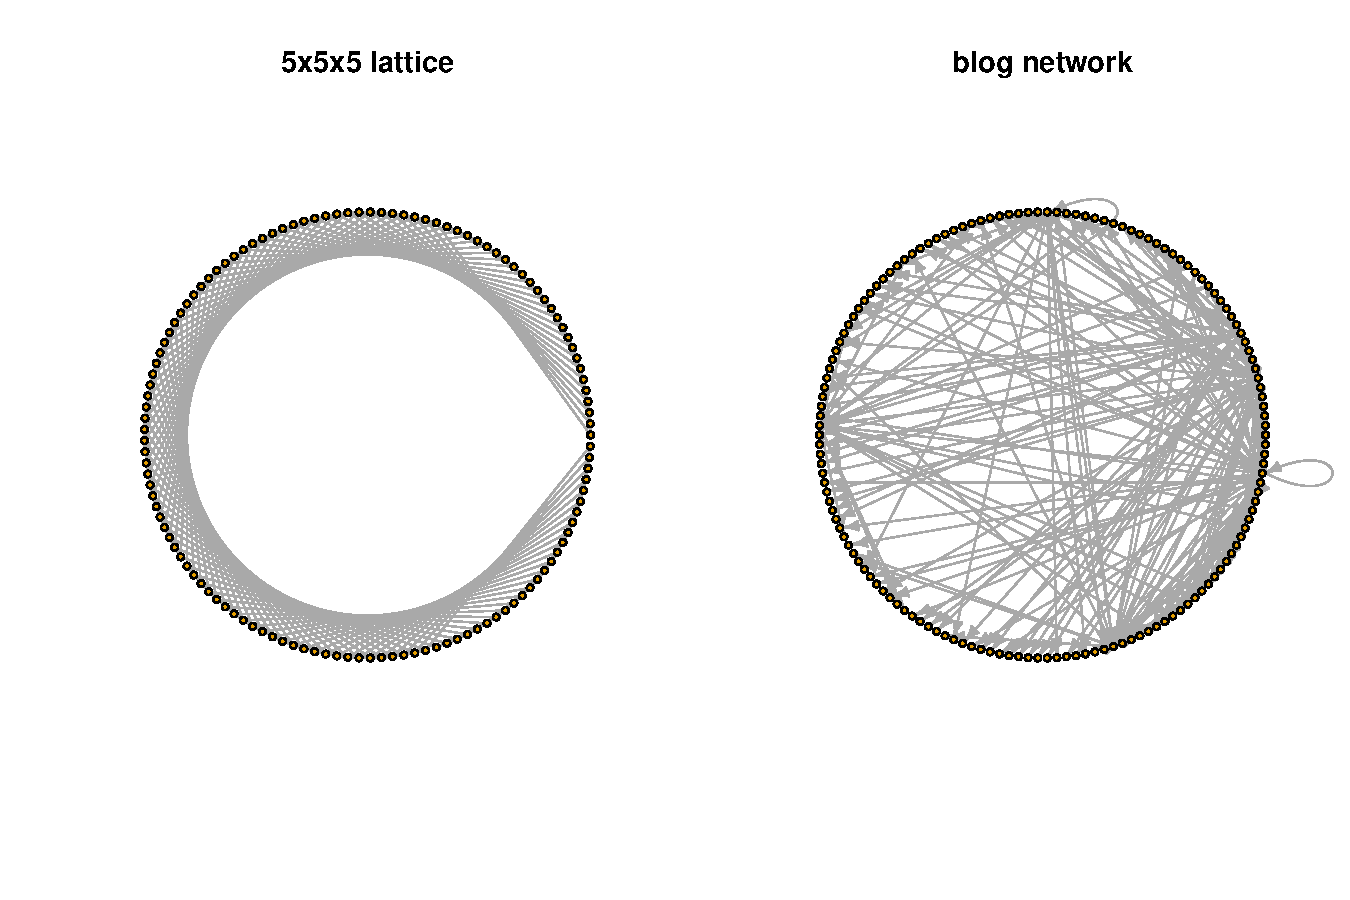
\includegraphics[width=.8\textwidth]{figures/vizu_3-1} 

\end{knitrout}
  
\end{frame}

\begin{frame}
  \frametitle{Layout and Vizualization}
  \framesubtitle{Example with Fruchterman and Reingold}

\begin{knitrout}\scriptsize
\definecolor{shadecolor}{rgb}{0.969, 0.969, 0.969}\color{fgcolor}\begin{kframe}
\begin{alltt}
\hlkwd{par}\hlstd{(}\hlkwc{mfrow}\hlstd{=}\hlkwd{c}\hlstd{(}\hlnum{1}\hlstd{,}\hlnum{2}\hlstd{))}

\hlkwd{plot}\hlstd{(GLattice,} \hlkwc{layout}\hlstd{=layout.fruchterman.reingold);} \hlkwd{title}\hlstd{(}\hlstr{"5x5x5 lattice"}\hlstd{)}

\hlkwd{plot}\hlstd{(GBlog   ,} \hlkwc{layout}\hlstd{=layout.fruchterman.reingold);} \hlkwd{title}\hlstd{(}\hlstr{"blog network"}\hlstd{)}
\end{alltt}
\end{kframe}
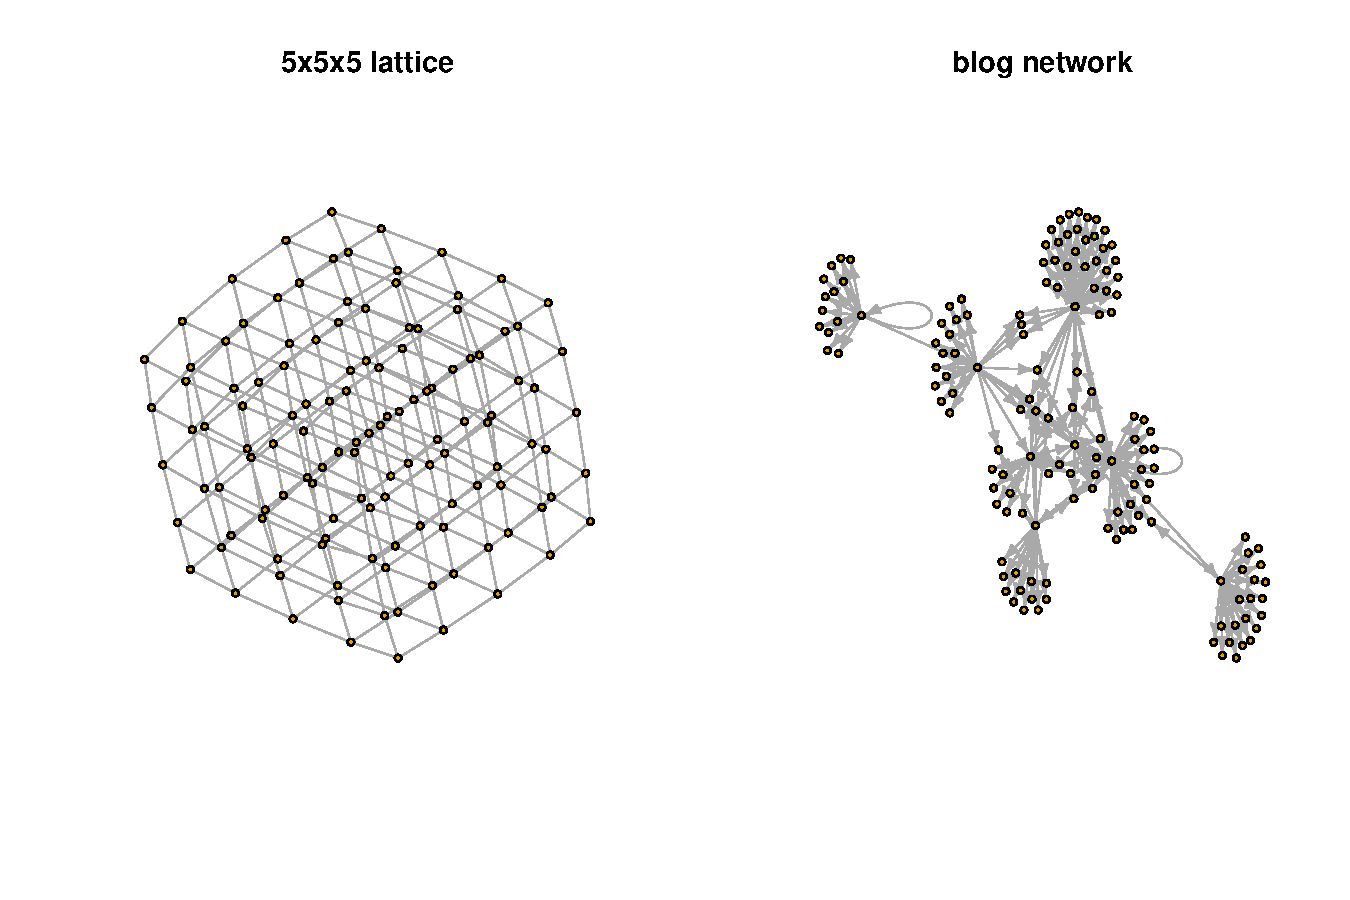
\includegraphics[width=.8\textwidth]{figures/vizu_4-1} 

\end{knitrout}
  
\end{frame}

\begin{frame}[fragile, allowframebreaks]
  \frametitle{Layout and Vizualization: \textbf{ggraph} way}
 
\begin{knitrout}\scriptsize
\definecolor{shadecolor}{rgb}{0.969, 0.969, 0.969}\color{fgcolor}\begin{kframe}
\begin{alltt}
\hlkwd{library}\hlstd{(ggraph)}
\hlkwd{library}\hlstd{(gridExtra)}
\hlstd{g1} \hlkwb{<-} \hlkwd{ggraph}\hlstd{(GBlog,} \hlkwc{layout} \hlstd{=} \hlstr{"fr"}\hlstd{)} \hlopt{+}
  \hlkwd{geom_edge_link}\hlstd{(}\hlkwc{color} \hlstd{=} \hlstr{"lightgray"}\hlstd{)} \hlopt{+} \hlkwd{geom_node_point}\hlstd{()} \hlopt{+} \hlkwd{theme_void}\hlstd{()}

\hlstd{g2} \hlkwb{<-} \hlkwd{ggraph}\hlstd{(GBlog   ,} \hlkwc{layout} \hlstd{=} \hlstr{"kk"}\hlstd{)} \hlopt{+}
  \hlkwd{geom_edge_link}\hlstd{(}\hlkwc{color} \hlstd{=} \hlstr{"lightgray"}\hlstd{)} \hlopt{+} \hlkwd{geom_node_point}\hlstd{()} \hlopt{+} \hlkwd{theme_void}\hlstd{()}

\hlstd{g3} \hlkwb{<-} \hlkwd{ggraph}\hlstd{(GBlog,} \hlkwc{layout} \hlstd{=} \hlstr{"linear"}\hlstd{)} \hlopt{+}
  \hlkwd{geom_edge_arc}\hlstd{(}\hlkwd{aes}\hlstd{(}\hlkwc{alpha}\hlstd{=..index..),} \hlkwc{show.legend} \hlstd{=} \hlnum{FALSE}\hlstd{)} \hlopt{+}
  \hlkwd{geom_node_point}\hlstd{()} \hlopt{+} \hlkwd{theme_void}\hlstd{()}

\hlstd{g4} \hlkwb{<-} \hlkwd{ggraph}\hlstd{(GBlog   ,} \hlkwc{layout} \hlstd{=} \hlstr{"linear"}\hlstd{,} \hlkwc{circular} \hlstd{=} \hlnum{TRUE}\hlstd{)} \hlopt{+}
  \hlkwd{geom_edge_link}\hlstd{(}\hlkwd{aes}\hlstd{(}\hlkwc{alpha}\hlstd{=..index..),} \hlkwc{show.legend} \hlstd{=} \hlnum{FALSE}\hlstd{)} \hlopt{+}
  \hlkwd{geom_node_point}\hlstd{()} \hlopt{+} \hlkwd{theme_void}\hlstd{()}

\hlkwd{grid.arrange}\hlstd{(g1, g2, g3, g4,} \hlkwc{nrow} \hlstd{=} \hlnum{2}\hlstd{,} \hlkwc{ncol} \hlstd{=} \hlnum{2}\hlstd{)}
\end{alltt}
\end{kframe}
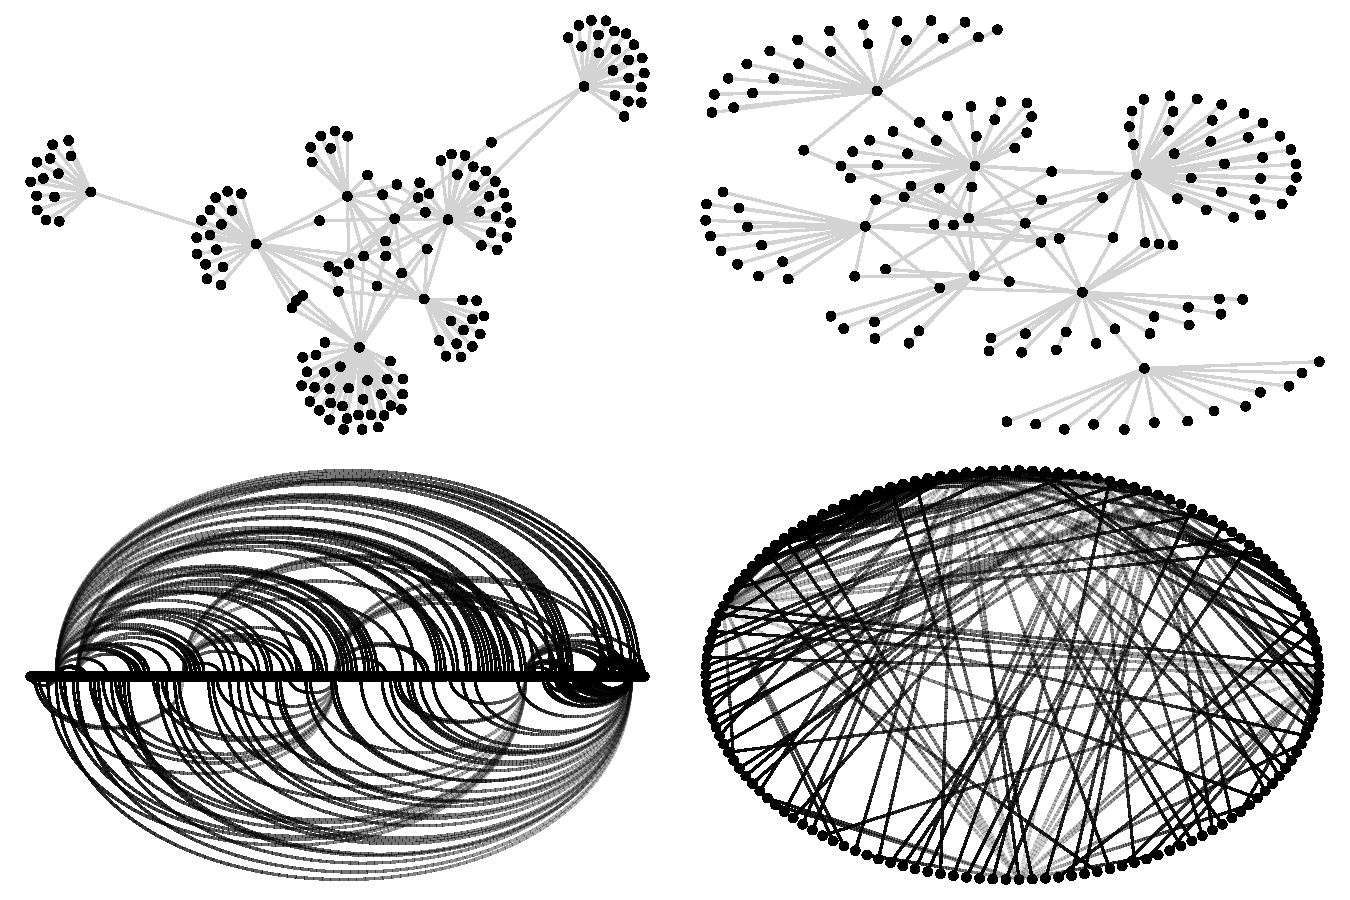
\includegraphics[width=.8\textwidth]{figures/ggraph_vizu_1-1} 

\end{knitrout}
\end{frame}

%% ==========================================================================
\section{Graph Partionning}
%% ==========================================================================

\begin{frame} 
  \frametitle{References}

    \begin{thebibliography}{99}
      \setbeamertemplate{bibliography item}[book]

    \bibitem[EK2]{EK2} Statistical Analysis of Network Data: Methods and Models,
    \newblock \textcolor{black}{Eric Kolazcyk}
    \newblock \alert{Chapiter 4, Section 4}

    \bibitem[CM1]{CM1} Analyse statistique de graphes, 
    \newblock \textcolor{black}{Catherine Matias}, \alert{Chapitre 3}

    \bibitem{DS}{DS} David Sontag's Lecture
    \newblock \url{http://people.csail.mit.edu/dsontag/courses/ml13/slides/lecture16.pdf}
    
    \bibitem[VLB]{VLB} A Tutorial on Spectral Clustering, 
    \newblock \textcolor{black}{Ulrike von Luxburg}

    \end{thebibliography}

\end{frame}

\begin{frame}
  \frametitle{Principle of graph partionning}

  \begin{definition}[Partition]
    A decomposition $\mathcal{C} = \{C_1,\dots,C_K\}$ of the vertices $\clV$ such that
    \begin{itemize}
      \item $C_k \cap C_{k'} = \emptyset$ for any $k\neq k'$
      \item $\bigcup_{k} C_k = \clV$
    \end{itemize}
  \end{definition}

  \vfill

  \begin{block}{Goal of graph partionning}
    Form a partition of the vertices with unsupervized approach where the $\mathcal{C}$ is composed by \alert{"cohesive"} sets of vertices, for instance,
    \begin{enumerate}
      \item vertices well connected among themselves
      \item well separated from the remaining vertices
    \end{enumerate}
    
  \end{block}

\end{frame}

%% ==========================================================================
\subsection{Hierarchical clustering}

\begin{frame}
  \frametitle{Principle}
  \framesubtitle{}


  \begin{algorithm}[H]
    \KwIn{$n$ individuals with $p$ attributes)}
    \BlankLine\BlankLine
    \DontPrintSemicolon
      1. Compute the dissimilarity between groups \;
      2. Regroup the two most similar elements \;
      
      Iterate until all element are in a single group \;
    \BlankLine\BlankLine
    \KwOut{$n$ nested partitions from $\set{\set{1},\dots,\set{n}}$ to $\set{\set{1,\dots,n}}$}

    \caption{Agglomerative hierarchical clustering}
  \end{algorithm}
  
  \begin{block}{Ingredients}
    \begin{enumerate}
      \item a dissimilarity measure between singleton
      \item a distance measure between sets
    \end{enumerate}
  \end{block}

\end{frame}

\begin{frame}
  \frametitle{Dissimilarity measures}

  \begin{block}{Standards}
    Use standard distances on adjacency matrix:
    \begin{itemize}
      \item Euclidean distance: $\displaystyle x_{ij} = \sqrt{\sum_{ij} (A_{ik} - A_{jk})^2} $
      \item Manhattan distance: $\displaystyle x_{ij} = \sum_{ij} |A_{ik} - A_{jk})| $
      \item  etc\dots
    \end{itemize}  
  \end{block}

  \vfill

  \begin{block}{Graph-specific}
    For instance,  Modularity (studied during tutorial)
  \end{block}
  
\end{frame}


\begin{frame}
  \frametitle{Example: karaté club}

\begin{knitrout}\scriptsize
\definecolor{shadecolor}{rgb}{0.969, 0.969, 0.969}\color{fgcolor}\begin{kframe}
\begin{alltt}
\hlkwd{library}\hlstd{(sand)}
\hlkwd{data}\hlstd{(karate)}

\hlkwd{par}\hlstd{(}\hlkwc{mfrow}\hlstd{=}\hlkwd{c}\hlstd{(}\hlnum{1}\hlstd{,}\hlnum{2}\hlstd{))}
\hlkwd{plot}\hlstd{(karate)}

\hlkwd{hist}\hlstd{(}\hlkwd{degree}\hlstd{(karate),} \hlkwc{col}\hlstd{=}\hlkwd{adjustcolor}\hlstd{(}\hlstr{"lightblue"}\hlstd{,} \hlkwc{alpha.f} \hlstd{=} \hlnum{0.5}\hlstd{),} \hlkwc{main}\hlstd{=}\hlstr{""}\hlstd{)}
\end{alltt}
\end{kframe}
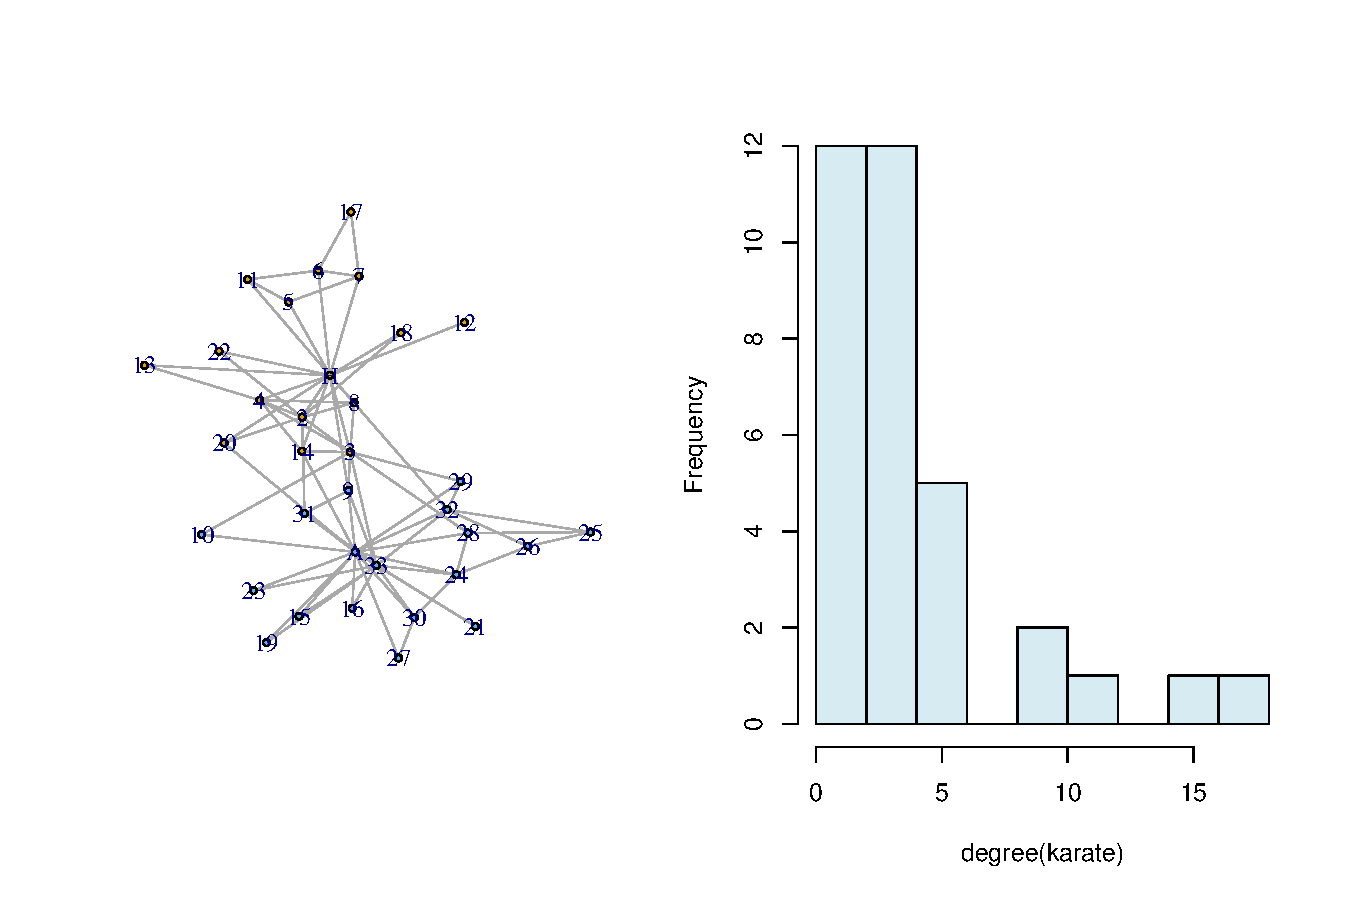
\includegraphics[width=.8\textwidth]{figures/degree_1-1} 

\end{knitrout}
      
\end{frame}


\begin{frame}[fragile,allowframebreaks]
  \frametitle{Examples of graph clustering}

\begin{knitrout}\scriptsize
\definecolor{shadecolor}{rgb}{0.969, 0.969, 0.969}\color{fgcolor}\begin{kframe}
\begin{alltt}
\hlstd{hc} \hlkwb{<-} \hlkwd{cluster_fast_greedy}\hlstd{(karate)}
\hlkwd{plot}\hlstd{(hc,karate)}
\end{alltt}
\end{kframe}
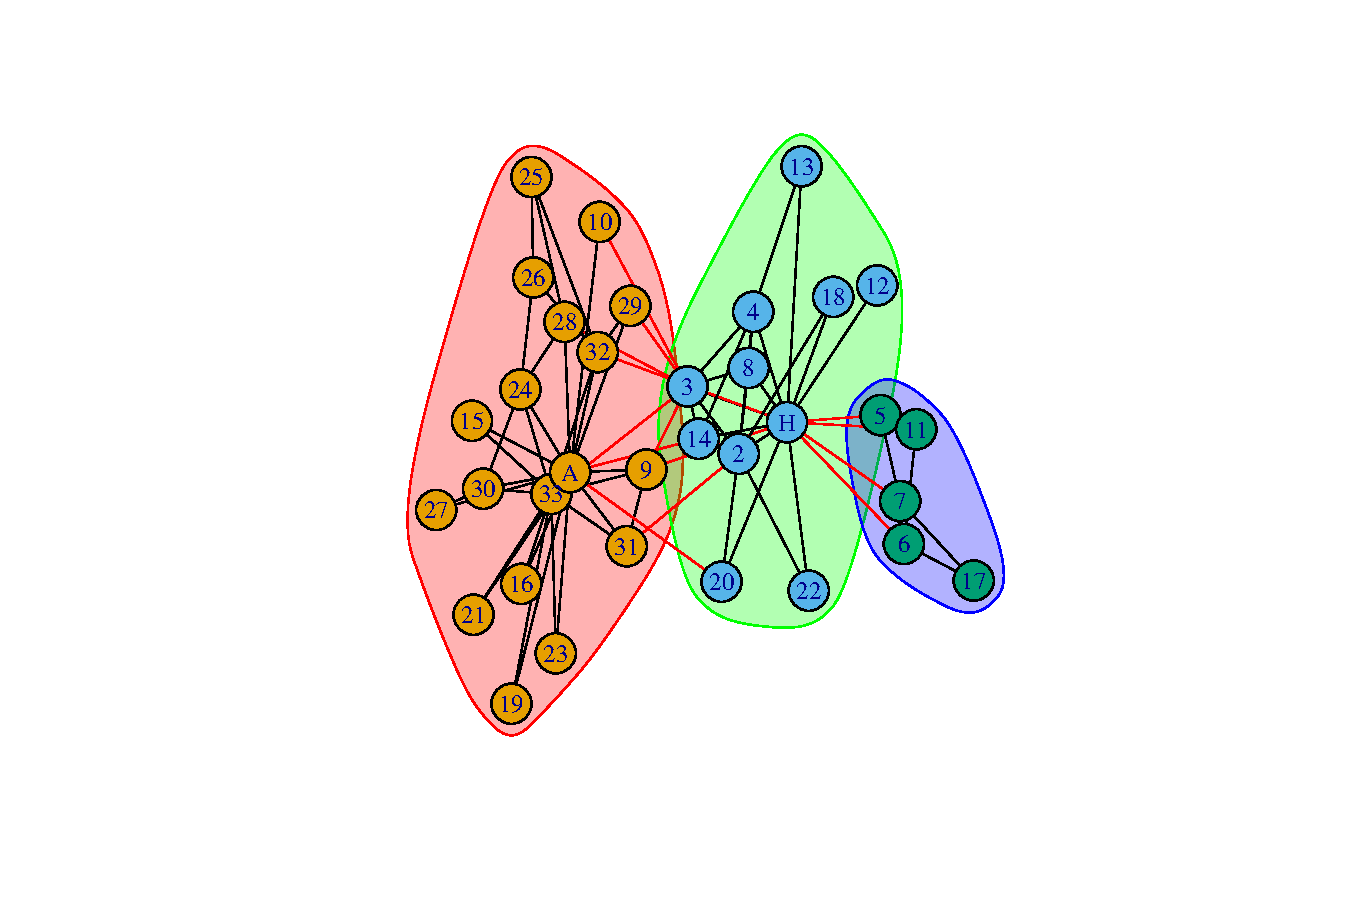
\includegraphics[width=.8\textwidth]{figures/unnamed-chunk-1-1} 

\end{knitrout}

\begin{knitrout}\scriptsize
\definecolor{shadecolor}{rgb}{0.969, 0.969, 0.969}\color{fgcolor}\begin{kframe}
\begin{alltt}
\hlstd{hc} \hlkwb{<-} \hlkwd{cluster_edge_betweenness}\hlstd{(karate)}
\hlkwd{plot}\hlstd{(hc,karate)}
\end{alltt}
\end{kframe}
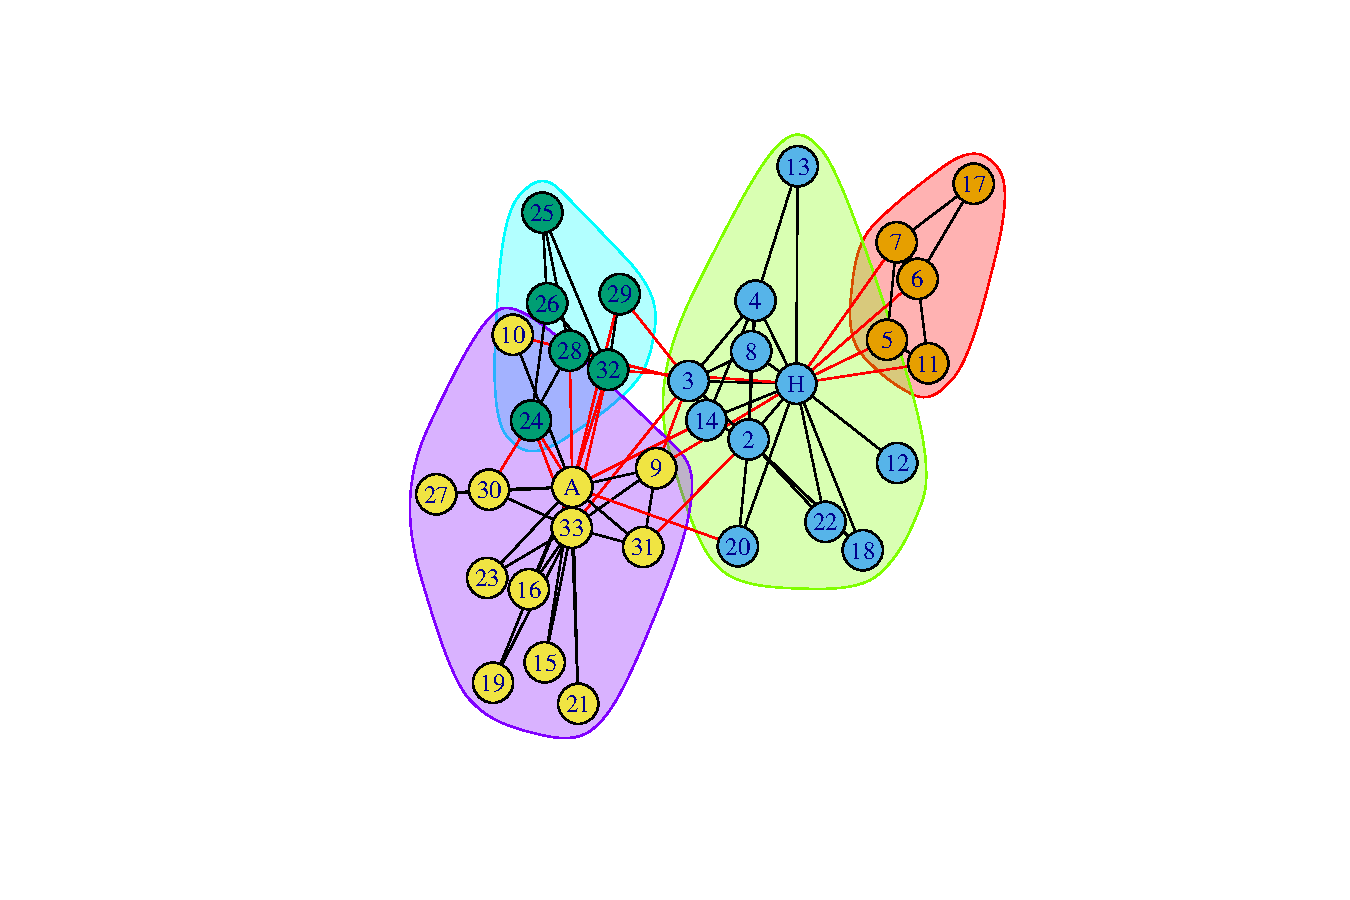
\includegraphics[width=.8\textwidth]{figures/unnamed-chunk-2-1} 

\end{knitrout}

\begin{knitrout}\scriptsize
\definecolor{shadecolor}{rgb}{0.969, 0.969, 0.969}\color{fgcolor}\begin{kframe}
\begin{alltt}
\hlstd{hc} \hlkwb{<-} \hlkwd{cluster_walktrap}\hlstd{(karate)}
\hlkwd{plot}\hlstd{(hc,karate)}
\end{alltt}
\end{kframe}
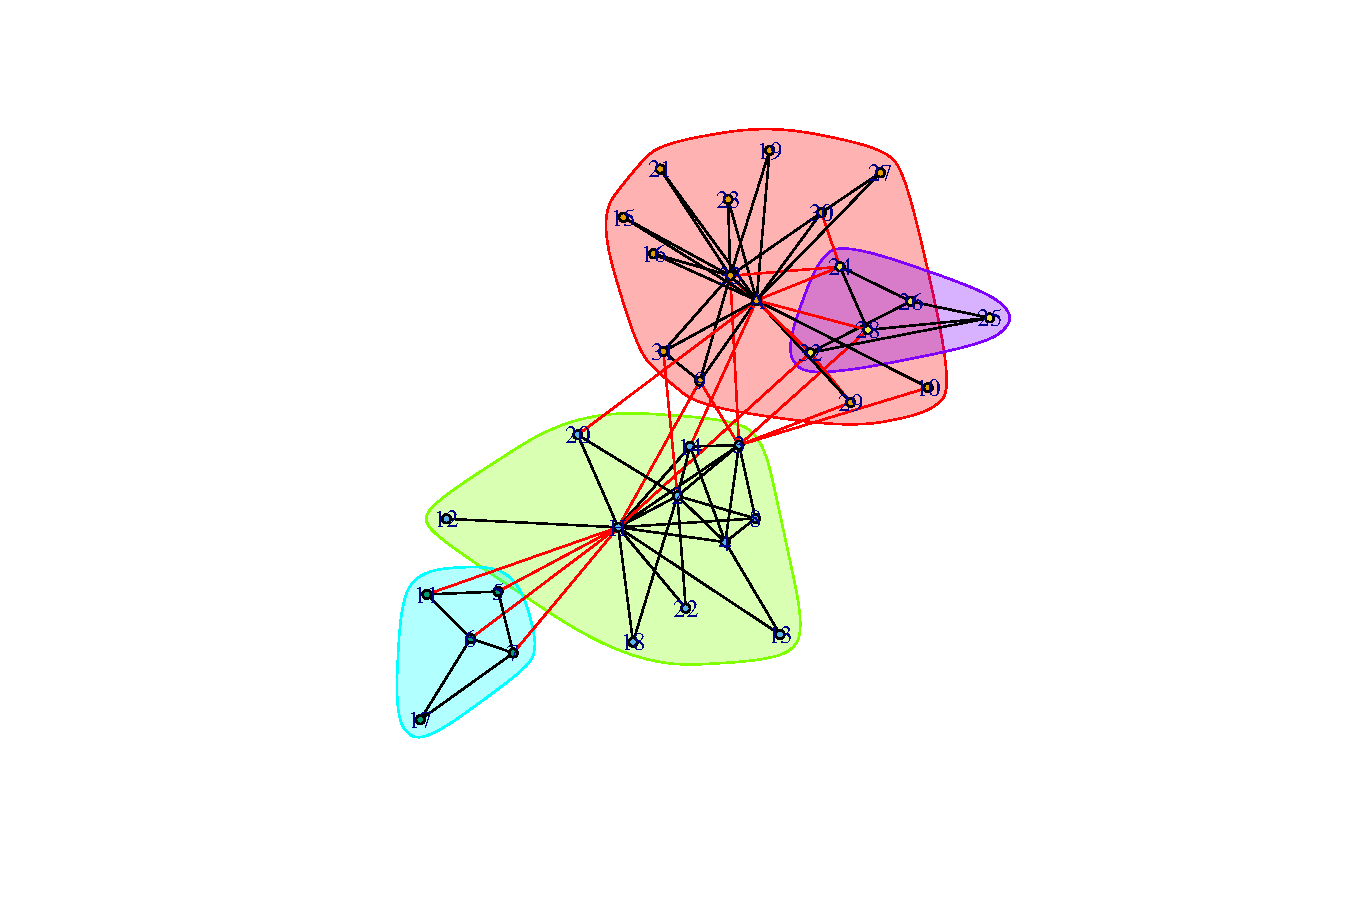
\includegraphics[width=.8\textwidth]{figures/unnamed-chunk-3-1} 

\end{knitrout}

\end{frame}

%% ==========================================================================
\subsection{Spectral Clustering}

\begin{frame}
  \frametitle{Graph Laplacian}

  \begin{definition}[(Un-normalized) Laplacian]
    The Laplacian matrix $\bL$, resulting from the modified incidence matrix $\tilde\bB$ $\tilde{\! B}_{ij}= 1/-1$ if $i$ is incident to $j$ as tail/head, is defined by 
    \[
      \bL = \tilde \bB \tilde \bB^\intercal = \bD - \bA,
    \]
    where $\bD = \diag(d_i, i\in\clV)$ is the diagonal matrix of degrees. 
  \end{definition}

  \begin{block}{Remark}
    \begin{itemize}
    \item $\bL$ is called Laplacian by analogy to the second order derivative (see below).
    \item Spectrum of $\bL$ has much to say about the structure of the graph $\clG$.
    \end{itemize}
  \end{block}

\end{frame}

\begin{frame}
  \frametitle{Graph Laplacian: spectrum}

  \begin{proposition}[Spectrum of $\bL$]
    The $n\times n$ matrix $\bL$ has the following properties:
    \[
      \bx^\top \bL \bx = \frac{1}{2} \sum_{i,j} A_{ij} (x_i - x_j)^2, \quad \forall \bx\in\Rset^n .
    \]
    \vspace{-.25cm}
    \begin{itemize}
      \item $\bL$ is a symmetric, positive semi-definite matrix,
      \item  the smallest eigenvalue is $0$ with associated eigenvector $\mathbf{1}$.
      \item $\bL$ has $n$ positive eigenvalues $0=\lambda_1<\dots <\lambda_n$. 
    \end{itemize}  
  \end{proposition}

  \begin{corollary}[Spectrum and Graph]
    \vspace{-.25cm}
    \begin{itemize}
      \item The multiplicity of the first eigen value ($0$) of $\bL$ determines the number of connected components in the graph.
      \item The larger the second non trivial eigenvalue, the higher the connectivity of $\clG$.
    \end{itemize}  
  \end{corollary}

\end{frame}

\begin{frame}
  \frametitle{Some variants}

  \begin{definition}[(Normalized) Laplacian]
    The normalized Laplacian matrix $\bL$ is defined by 
    \[
      \bL_N = \bD^{-1/2}\bL\bD^{-1/2} = \bI - \bD^{-1/2} \bA \bD^{-1/2}.
    \]
  \end{definition}
  
  \vfill

  \begin{definition}[(Absolute) Graph Laplacian]
    The absolute Laplacian matrix $\bL_{abs}$ is defined by 
    \[
      \bL_{abs} = \bD^{-1/2}\bA\bD^{-1/2} = \bI - \bL_N,
    \]
    with eigenvalues $1-\lambda_n \leq \dots \leq 1-\lambda_2 \leq 1-\lambda_1 = 1$, where $0=\lambda_1\leq \dots \leq \lambda_n$ are the eigenvalues of $\bL_N$.
  \end{definition}

\end{frame}

\begin{frame}
  \frametitle{Spectral Clustering}
    
  \begin{block}{Principle}
  
  \begin{enumerate}
    \item Use the spectral property of $\bL$ to perform clustering in the eigen space \medskip
    \item If the network have $K$ connected components, the first $K$ eigenvectors are $\mathbf{1}$ span the eigenspace associated with eigenvalue $0$ \medskip
    \item Applying a simple clustering algorithm to the rows of the $K$ first eigenvectors separate the components
  \end{enumerate}
  $\rightsquigarrow$ This principle generalizes to a graph with a single component: spectral clustering tends to separates groups of nodes which are highly connected together
  
  \end{block}
  
\end{frame}

\begin{frame}
  \frametitle{Normalized Spectral Clustering}
  \framesubtitle{by Ng, Jordan and Weiss (2002)}

\begin{algorithm}[H]
  \KwIn{Adjacency matrix and number of classes $Q$}
  \BlankLine\BlankLine
  \DontPrintSemicolon
  
  Compute the normalized graph Laplacian $\mathbf{L}$\;
  Compute the eigen vectors of $\mathbf{L}$ associated with the $Q$ \alert{smallest eigenvalues}\;
  Define $\mathbf{U}$,  the $n\times Q$ matrix  that encompasses these $Q$ vectors \;
  Define $\tilde{\mathbf{U}}$, the row-wise normalized version of $\mathbf{U}$: $ \tilde{u}_{ij} = \frac{u_{ij}}{\| \mathbf{U}_i\|_2}$\;
  Apply k-means to $(\tilde{\mathbf{U}}_i)_{i=1,\dots,n}$

  \BlankLine\BlankLine
  \KwOut{vector of classes $\mathbf{C}\in \mathcal{Q}^n$, such as  $C_i = q$ if $i\in q$}

\end{algorithm}

  \vfill

  \begin{block}{Remarks}
    \begin{itemize}
      \item implemented during today's lab
      \item also apply to no graphical data!
    \end{itemize}
  \end{block}
  
\end{frame}

% \begin{frame}
%   \frametitle{Absolute Spectral Clustering}
% 
% \begin{algorithm}[H]
%   \KwIn{Adjacency matrix and number of classes $Q$}
%   \BlankLine\BlankLine
%   \DontPrintSemicolon
%   
%   Compute the graph Laplacian $\mathbf{L}_{abs}$\;
%   Compute the eigen vectors of $\mathbf{L}_{abs}$ associated with the $Q$ \alert{largest} absolute eigenvalues\;
%   Define $\mathbf{U}$,  the $p\times Q$ matrix  that encompasses these $Q$ vectors \;
%   Apply k-means to $(\mathbf{U}_i)_{i=1,\dots,p}$
% 
%   \BlankLine\BlankLine
%   \KwOut{vector of classes $\mathbf{C}\in \mathcal{Q}^p$, such as  $C_i = q$ if $i\in q$}
% 
%   \caption{Spectral Clustering by Rohe et al. (2011)}
% \end{algorithm}
% 
% \end{frame}

\begin{frame}[fragile,allowframebreaks]
  \frametitle{Example: Karate club and Fielder vector and eigenvalue}

\begin{knitrout}\scriptsize
\definecolor{shadecolor}{rgb}{0.969, 0.969, 0.969}\color{fgcolor}\begin{kframe}
\begin{alltt}
\hlstd{eigen_karate} \hlkwb{<-} \hlkwd{graph.laplacian}\hlstd{(karate)} \hlopt \hlkwd{eigen}\hlstd{()}

\hlstd{fielder_vector} \hlkwb{<-} \hlstd{eigen_karate}\hlopt{$}\hlstd{vectors[, igraph}\hlopt{::}\hlkwd{vcount}\hlstd{(karate)} \hlopt{-} \hlnum{1}\hlstd{]}
\hlstd{faction} \hlkwb{<-} \hlkwd{as.character}\hlstd{(}\hlkwd{vcount}\hlstd{(karate))}
\hlstd{faction[}\hlkwd{V}\hlstd{(karate)}\hlopt{$}\hlstd{Faction} \hlopt{==} \hlnum{1}\hlstd{]} \hlkwb{<-} \hlstr{"red"}
\hlstd{faction[}\hlkwd{V}\hlstd{(karate)}\hlopt{$}\hlstd{Faction} \hlopt{==} \hlnum{2}\hlstd{]} \hlkwb{<-} \hlstr{"cyan"}

\hlkwd{par}\hlstd{(}\hlkwc{mfrow} \hlstd{=} \hlkwd{c}\hlstd{(}\hlnum{1}\hlstd{,}\hlnum{2}\hlstd{))}
\hlkwd{plot}\hlstd{(eigen_karate}\hlopt{$}\hlstd{values,} \hlkwc{col} \hlstd{=} \hlstr{"blue"}\hlstd{,} \hlkwc{ylab} \hlstd{=} \hlstr{"Eigenvalues of Graph Laplacian"}\hlstd{)}
\hlkwd{plot}\hlstd{(fielder_vector,} \hlkwc{pch} \hlstd{=} \hlnum{16}\hlstd{,} \hlkwc{xlab} \hlstd{=} \hlstr{"labels"}\hlstd{,}
   \hlkwc{ylab} \hlstd{=} \hlstr{"Fiedler vector entry"}\hlstd{,} \hlkwc{col} \hlstd{= faction)}
\hlkwd{abline}\hlstd{(}\hlnum{0}\hlstd{,} \hlnum{0}\hlstd{,} \hlkwc{lwd} \hlstd{=} \hlnum{2}\hlstd{,} \hlkwc{col} \hlstd{=} \hlstr{"lightgray"}\hlstd{)}
\end{alltt}
\end{kframe}
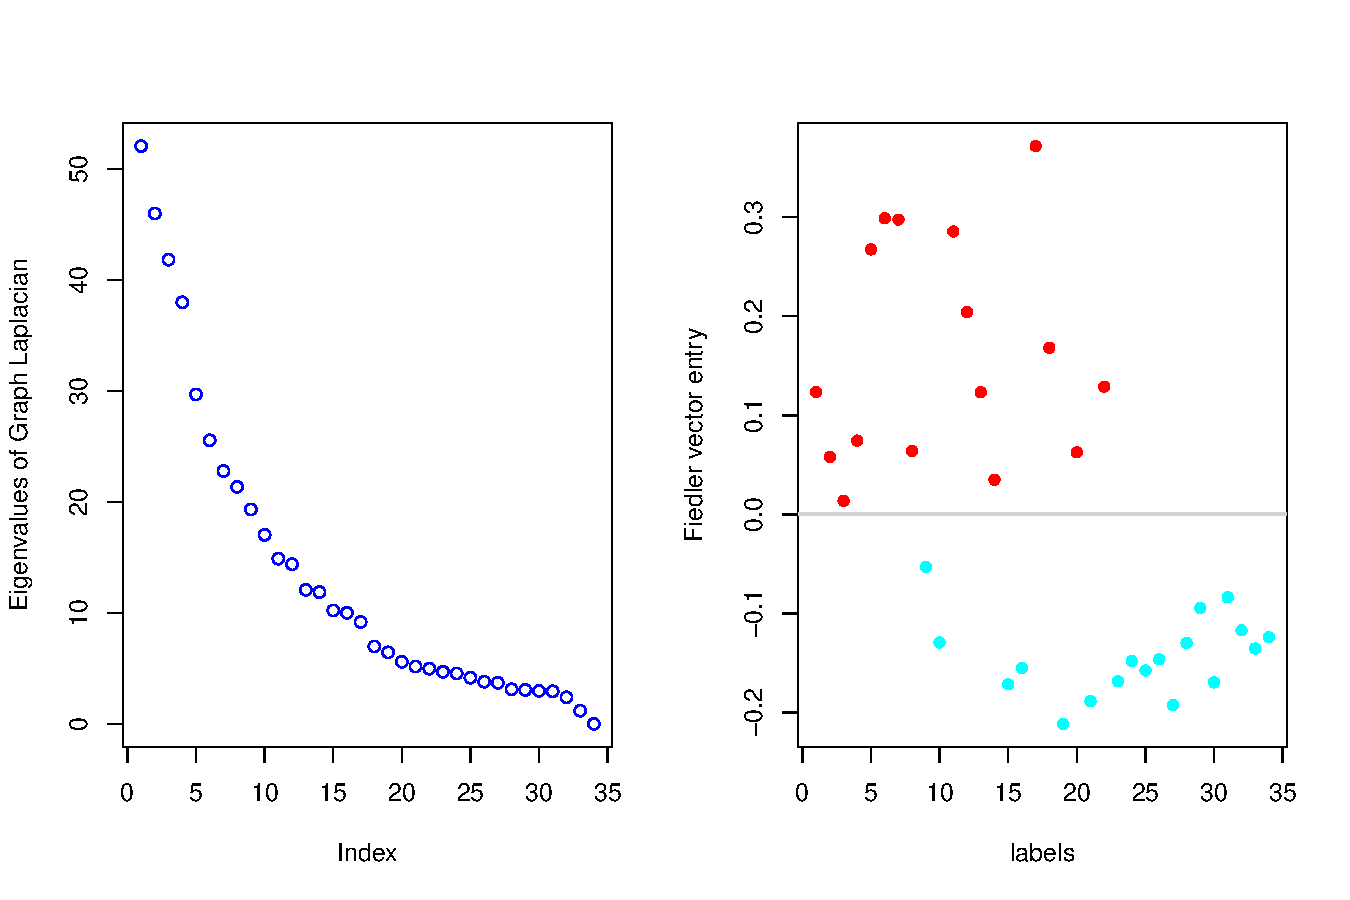
\includegraphics[width=.8\textwidth]{figures/laplacian_example-1} 

\end{knitrout}

\end{frame}

\begin{frame}[fragile]
  \frametitle{Clustering based on the first non null eigenvalue}
  
\begin{knitrout}\scriptsize
\definecolor{shadecolor}{rgb}{0.969, 0.969, 0.969}\color{fgcolor}\begin{kframe}
\begin{alltt}
\hlstd{hc} \hlkwb{<-} \hlkwd{cluster_leading_eigen}\hlstd{(karate)}
\hlkwd{plot}\hlstd{(hc,karate)}
\end{alltt}
\end{kframe}
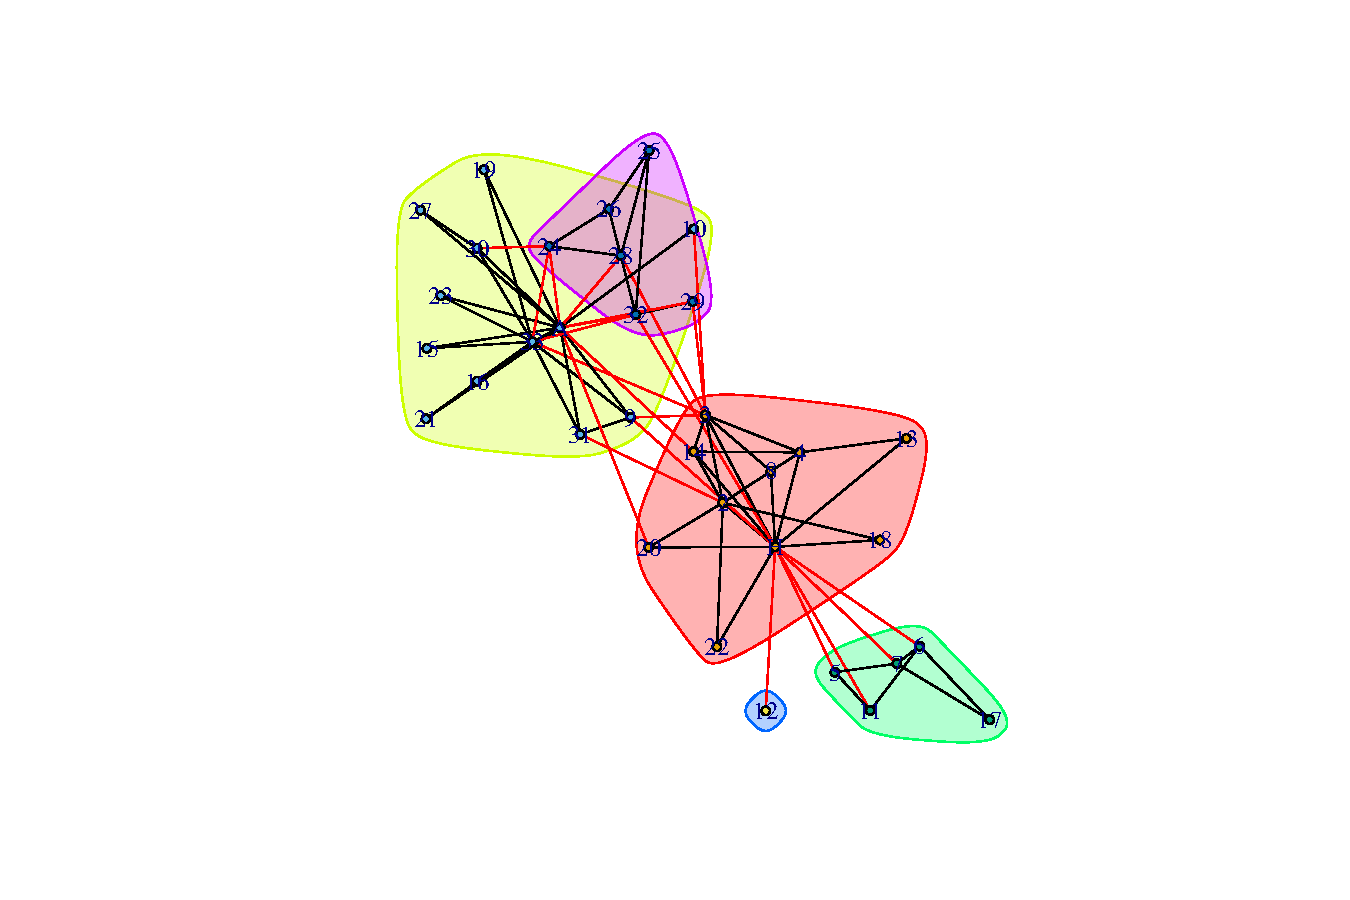
\includegraphics[width=.8\textwidth]{figures/unnamed-chunk-4-1} 

\end{knitrout}

\end{frame}

%% ==========================================================================
\section{The Stochastic Block Model (SBM)}
%% ==========================================================================

\begin{frame}
  \frametitle{References}

    \begin{thebibliography}{99}
      \setbeamertemplate{bibliography item}[book]

    \bibitem[EK2]{EK2} Statistical Analysis of Network Data: Methods and Models
    \newblock \textcolor{black}{Eric Kolazcyk}
    \newblock \alert{Chapters 5 and 6}

      \setbeamertemplate{bibliography item}[article]

    \bibitem[EK2]{EK2} Mixture model for random graphs, Statistics and Computing
    \newblock \textcolor{black}{Daudin, Robin, Picard}
    \newblock {\tiny\url{pbil.univ-lyon1.fr/members/fpicard/franckpicard_fichiers/pdf/DPR08.pdf
}}

    \bibitem[CM1]{CM1} Analyse statistique de graphes,
    \newblock \textcolor{black}{Catherine Matias}
    \newblock \alert{Chapitre 4, Section 4}

    \end{thebibliography}

\end{frame}

\begin{frame}
  \frametitle{Motivations}

  \begin{block}{Last section: \alert{find an underlying organization in a observed network}}
    Spectral or hierachical clustering for network data \\
    \begin{itemize}
      \item[$\rightsquigarrow$] \alert{Not model-based}, thus no statistical inference possible
    \end{itemize}
  \end{block}

  \begin{block}{Now: \alert{clustering of network based on a probabilistic model of the graph}}
    Become familiar with
    \begin{itemize}
      \item the stochastic block model, a random graph model tailored for clustering vertices,
      \item the variational EM algorithm used to infer SBM from network data.
    \end{itemize}
  \end{block}

  \onslide{
  \begin{center}
    hierarchical/kmeans clustering $\leftrightarrow$ \alert{Gaussian mixture models} \\
      $\Updownarrow$ \\
    hierarchical/spectral clustering for network $\leftrightarrow$ Stochastic block model
  \end{center}
  }

\end{frame}

%% ==========================================================================
\subsection{Some Graphs Models and their limitations}
%% ==========================================================================

\begin{frame}
  \frametitle{A mathematical model: Erdös-Rényi graph}

  \begin{definition}
    Let $\clV = {1,\dots,n}$ be a set of fixed vertices. The (simple) Erdös-Rény model $\mathcal{G}(n,\pi)$ assumes random edges between pairs of nodes with probability $\pi$. In orther word, the (random) adjacency matrix $\bX$ is such that
    \begin{equation*}
      X_{ij} \sim \mathcal{B}(\pi)
    \end{equation*}
  \end{definition}

  \vfill

  \begin{proposition}[degree distribution]
    The (random) degree $D_i$ of vertex $i$ follows a binomial distribution:
      \begin{equation*}
        D_i \sim b(n-1, \pi).
      \end{equation*}
  \end{proposition}

\end{frame}

\begin{frame}[fragile]
  \frametitle{Erdös-Rényi - example}

\begin{knitrout}\scriptsize
\definecolor{shadecolor}{rgb}{0.969, 0.969, 0.969}\color{fgcolor}\begin{kframe}
\begin{alltt}
\hlstd{G1} \hlkwb{<-} \hlstd{igraph}\hlopt{::}\hlkwd{sample_gnp}\hlstd{(}\hlnum{10}\hlstd{,} \hlnum{0.1}\hlstd{)}
\hlstd{G2} \hlkwb{<-} \hlstd{igraph}\hlopt{::}\hlkwd{sample_gnp}\hlstd{(}\hlnum{10}\hlstd{,} \hlnum{0.9}\hlstd{)}
\hlstd{G3} \hlkwb{<-} \hlstd{igraph}\hlopt{::}\hlkwd{sample_gnp}\hlstd{(}\hlnum{100}\hlstd{,} \hlnum{.02}\hlstd{)}
\hlkwd{par}\hlstd{(}\hlkwc{mfrow}\hlstd{=}\hlkwd{c}\hlstd{(}\hlnum{1}\hlstd{,}\hlnum{3}\hlstd{))}
\hlkwd{plot}\hlstd{(G1,} \hlkwc{vertex.label}\hlstd{=}\hlnum{NA}\hlstd{) ;} \hlkwd{plot}\hlstd{(G2,} \hlkwc{vertex.label}\hlstd{=}\hlnum{NA}\hlstd{)}
\hlkwd{plot}\hlstd{(G3,} \hlkwc{vertex.label}\hlstd{=}\hlnum{NA}\hlstd{,} \hlkwc{layout}\hlstd{=layout.circle)}
\end{alltt}
\end{kframe}
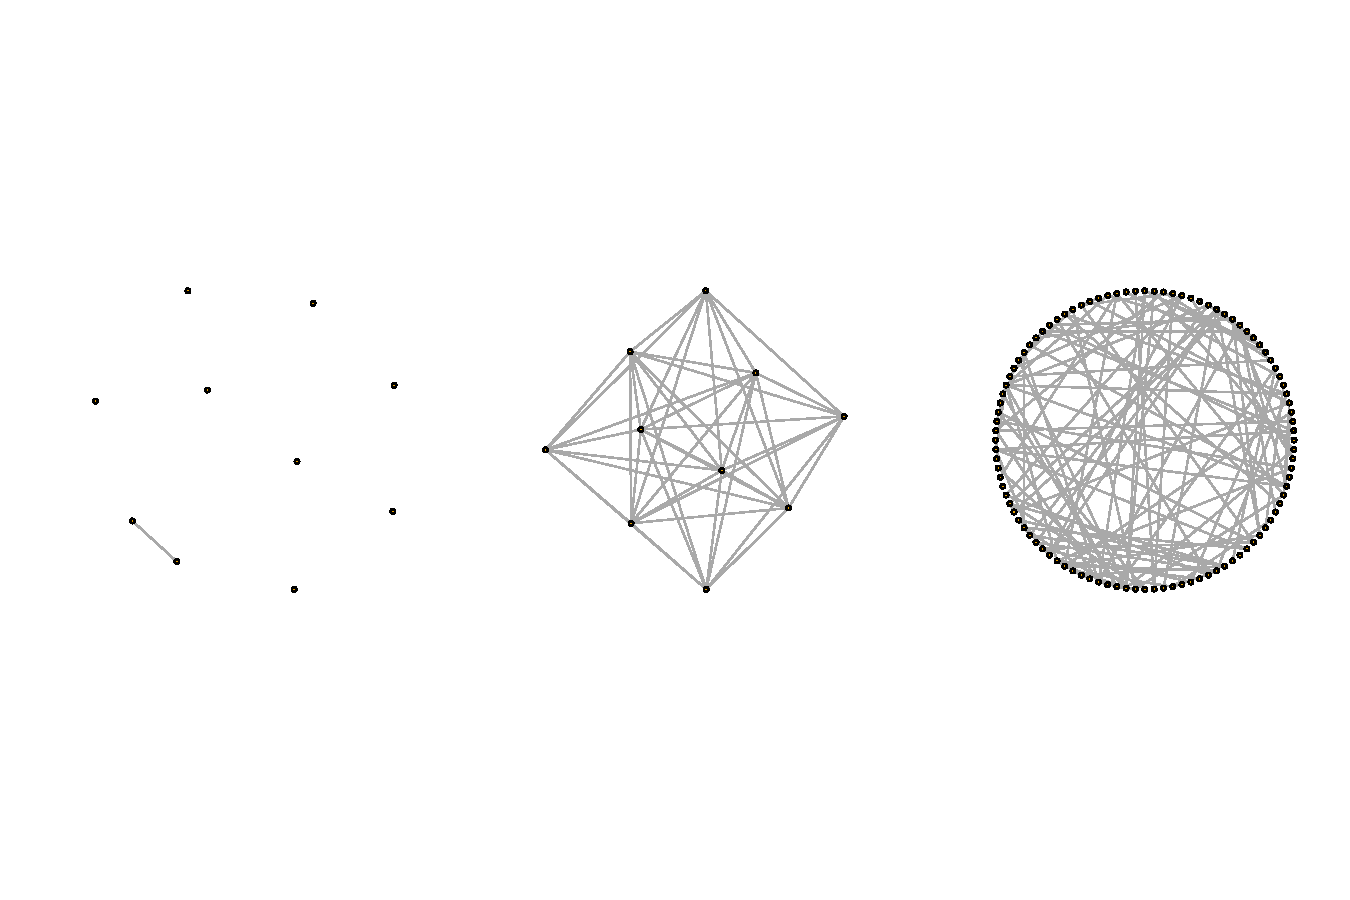
\includegraphics[width=.8\textwidth]{figures/ER_example-1} 

\end{knitrout}
\end{frame}

\begin{frame}[fragile]
  \frametitle{Erdös-Rény - limitations: very homegeneous}

\begin{knitrout}\scriptsize
\definecolor{shadecolor}{rgb}{0.969, 0.969, 0.969}\color{fgcolor}\begin{kframe}
\begin{alltt}
\hlkwd{average.path.length}\hlstd{(G3);} \hlkwd{diameter}\hlstd{(G3)}
\end{alltt}
\begin{verbatim}
## [1] 5.834998
## [1] 14
\end{verbatim}
\end{kframe}
\end{knitrout}

\begin{knitrout}\scriptsize
\definecolor{shadecolor}{rgb}{0.969, 0.969, 0.969}\color{fgcolor}
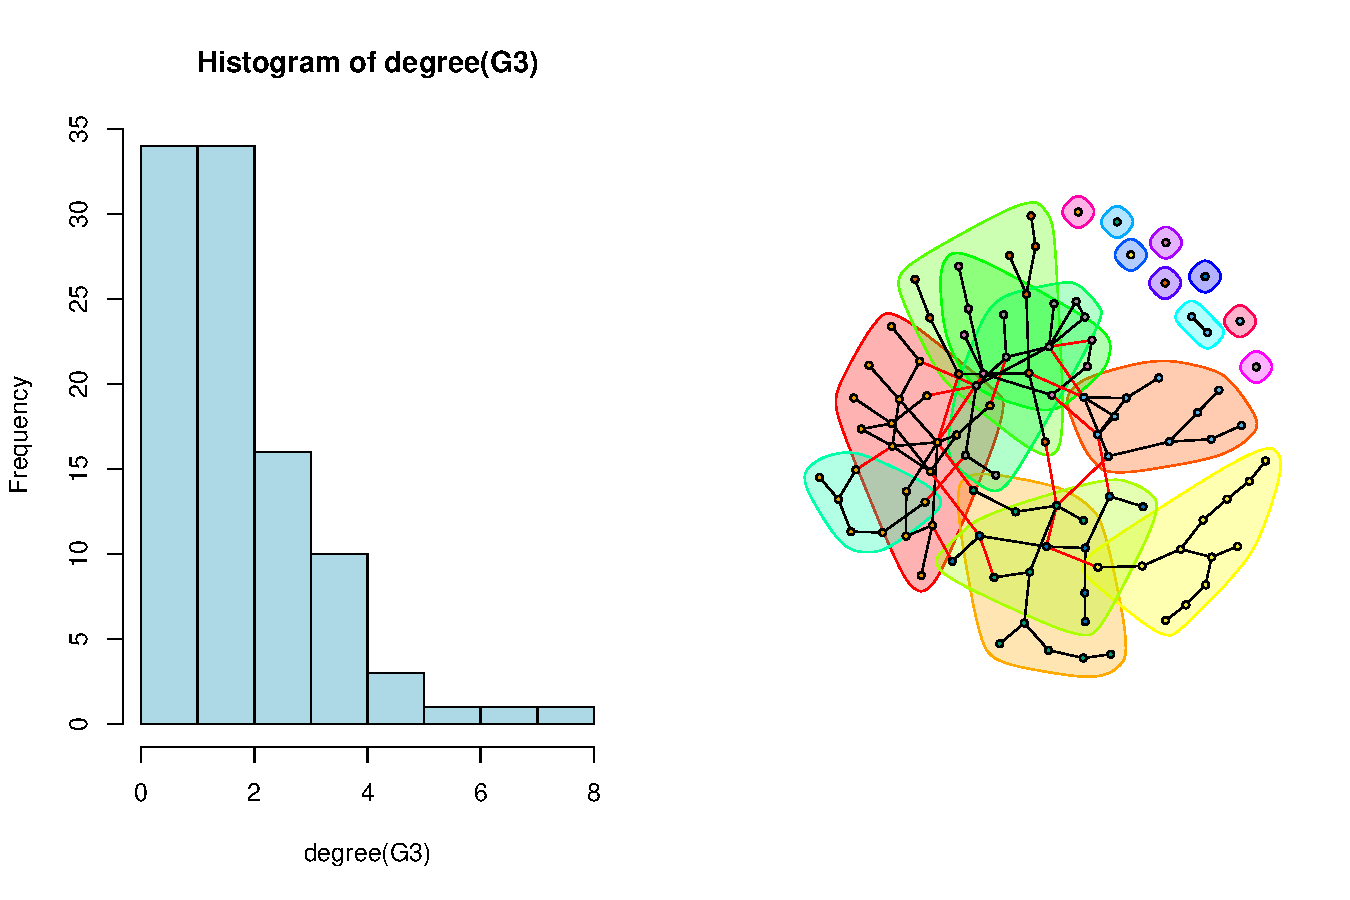
\includegraphics[width=.8\textwidth]{figures/ER_limitation2-1} 

\end{knitrout}
\end{frame}

\begin{frame}
  \frametitle{Mechanism-based model: preferential attachment}

  The graph is defined dynamically as follows
  \begin{block}{Definition}
    Start from a initial graph $\mathcal{G}_0 = (\mathcal{V}_0,\mathcal{E}_0)$, then for each time step,
    \begin{enumerate}
      \item At $t$ a new node $V_t$ is added
      \item $V_t$ is connected to $i \in V_{t-1}$ with probability
      \begin{equation*}
        D_i^\alpha + \mathrm{cst.}
      \end{equation*}
    \end{enumerate}
  \end{block}
  $\rightsquigarrow$ Nodes with high degree get more connections thus \alert{richers get richers}
\end{frame}

\begin{frame}[fragile]
  \frametitle{Preferential attachment - example}

\begin{knitrout}\scriptsize
\definecolor{shadecolor}{rgb}{0.969, 0.969, 0.969}\color{fgcolor}\begin{kframe}
\begin{alltt}
\hlstd{G1} \hlkwb{<-} \hlstd{igraph}\hlopt{::}\hlkwd{sample_pa}\hlstd{(}\hlnum{20}\hlstd{,} \hlnum{1}\hlstd{,} \hlkwc{directed}\hlstd{=}\hlnum{FALSE}\hlstd{)}
\hlstd{G2} \hlkwb{<-} \hlstd{igraph}\hlopt{::}\hlkwd{sample_pa}\hlstd{(}\hlnum{20}\hlstd{,} \hlnum{5}\hlstd{,} \hlkwc{directed}\hlstd{=}\hlnum{FALSE}\hlstd{)}
\hlstd{G3} \hlkwb{<-} \hlstd{igraph}\hlopt{::}\hlkwd{sample_pa}\hlstd{(}\hlnum{200}\hlstd{,} \hlkwc{directed}\hlstd{=}\hlnum{FALSE}\hlstd{)}
\hlkwd{par}\hlstd{(}\hlkwc{mfrow}\hlstd{=}\hlkwd{c}\hlstd{(}\hlnum{1}\hlstd{,}\hlnum{3}\hlstd{))}
\hlkwd{plot}\hlstd{(G1,} \hlkwc{vertex.label}\hlstd{=}\hlnum{NA}\hlstd{) ;} \hlkwd{plot}\hlstd{(G2,} \hlkwc{vertex.label}\hlstd{=}\hlnum{NA}\hlstd{)}
\hlkwd{plot}\hlstd{(G3,} \hlkwc{vertex.label}\hlstd{=}\hlnum{NA}\hlstd{,} \hlkwc{layout}\hlstd{=layout.circle)}
\end{alltt}
\end{kframe}
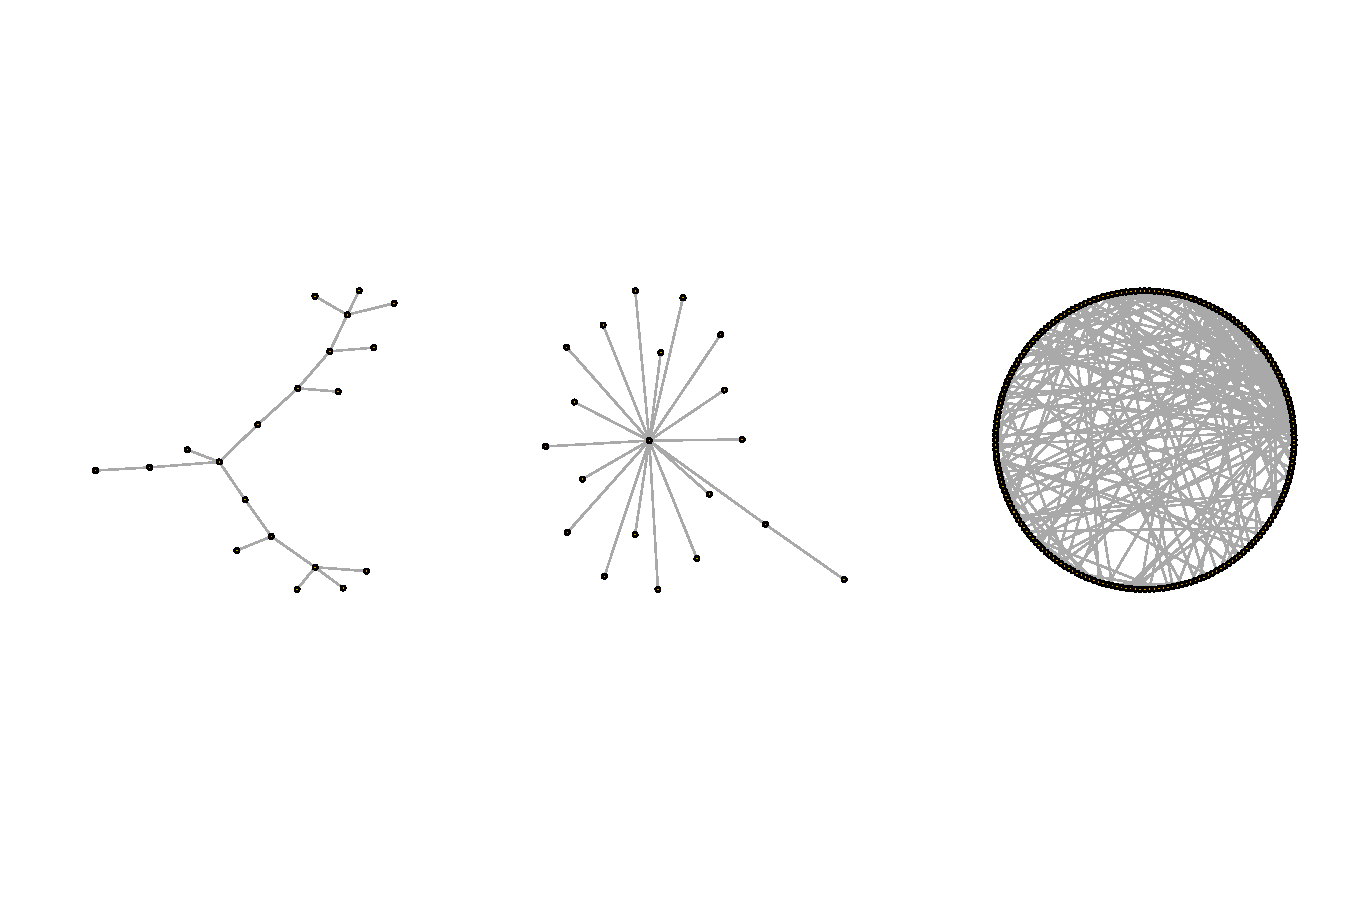
\includegraphics[width=.8\textwidth]{figures/PA_example-1} 

\end{knitrout}

\end{frame}

\begin{frame}[fragile]
  \frametitle{Preferential attachment - limitations}

\begin{knitrout}\scriptsize
\definecolor{shadecolor}{rgb}{0.969, 0.969, 0.969}\color{fgcolor}\begin{kframe}
\begin{alltt}
\hlkwd{average.path.length}\hlstd{(G3);} \hlkwd{diameter}\hlstd{(G3)}
\end{alltt}
\begin{verbatim}
## [1] 6.137487
## [1] 14
\end{verbatim}
\end{kframe}
\end{knitrout}

\begin{knitrout}\scriptsize
\definecolor{shadecolor}{rgb}{0.969, 0.969, 0.969}\color{fgcolor}
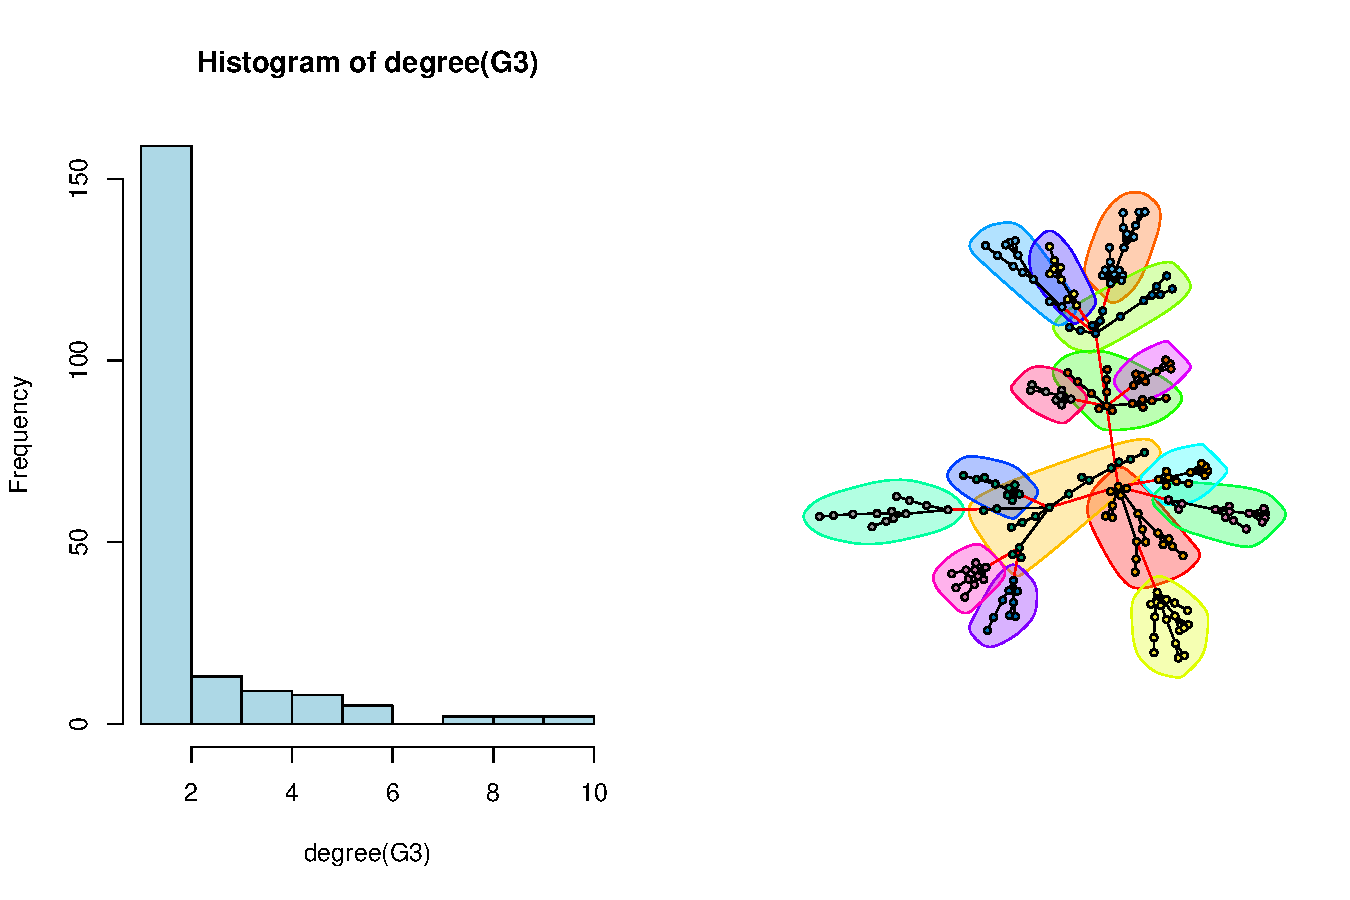
\includegraphics[width=.8\textwidth]{figures/PA_limitation2-1} 

\end{knitrout}
\end{frame}

\begin{frame}
  \frametitle{Limitations}

    \begin{itemize}
    \item \alert{Erdös-Rényi}\\
      The ER model does not fit well real world network
      \begin{itemize}
        \item As can been seen from its degree distribution
        \item ER is generally too homogeneous
      \end{itemize}
    \item \alert{Preferential attachment}
      \begin{itemize}
        \item Is defined through an algorithm so performing statistics is complicated
        \item Is stucked to the power-law distribution of degrees
      \end{itemize}
    \end{itemize}

  \vfill

  \begin{block}{The Stochastic Block Model}
    The SBM\footnote{Other models exist (e.g. exponential model for random graphs) but less popular.} generalizes ER in a mixture framework. It provides
    \begin{itemize}
      \item a statistical framework to adjust and interpret the parameters
      \item a flexible yet simple specification that fits many existing network data
    \end{itemize}
  \end{block}

\end{frame}


%% ==========================================================================
\subsection{Mixture of Erdös-Rényi and the SBM}
%% ==========================================================================

\begin{frame}
  \frametitle{Stochastic Block Model: definition}
    \framesubtitle{Mixture model point of view: mixture of Erdös-Rényi}

    \begin{block}{Latent structure}
      Let $\mathcal{V} = \set{1,..,n}$ be a fixed set of vertices. We give each $i\in\mathcal{V}$ a \alert{latent label} among a set $\mathcal{Q}=\{1,\dots,Q\}$ such that
    \begin{itemize}
    \item $\alpha_q = \prob(i\in q), \quad \sum_q \alpha_q=1$;
    \item $Z_{iq}=\1_{\{i \in  q\}}$  are independent  hidden variables.
   \end{itemize}
   \end{block}

    \begin{block}{The conditional distribution of the edges}
    Connexion probabilities depend on the node class belonging:
    \begin{equation*}
      X_{ij} | \set{i\in q, j\in\ell} \sim \mathcal{B}(\pi_{q \ell}) \qquad \bigg(\Leftrightarrow       X_{ij} | \set{Z_{iq}Z_{j\ell}=1} \sim \mathcal{B}(\pi_{q \ell}).
 \bigg)
    \end{equation*}
    The $Q\times Q$ matrix ${\boldsymbol\pi}$  gives for all couple of labels $\pi_{q\ell}=\mathbb{P}(X_{ij}=1|i\in q, j\in\ell)$.
   \end{block}

\end{frame}


\begin{frame}
  \frametitle{Stochastic Block Model: the big picture}

  \begin{center}
    \begin{overlayarea}{\textwidth}{.5\textheight}
      \begin{columns}
        \begin{column}{.45\paperwidth}
        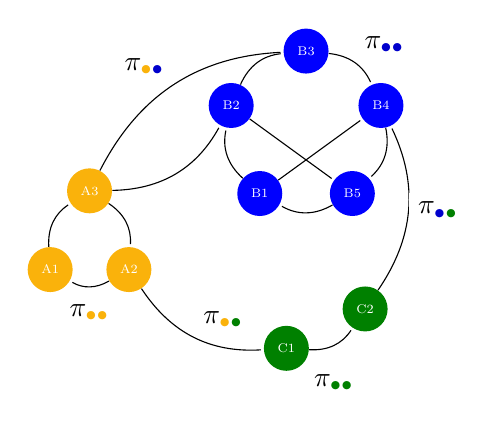
\begin{tikzpicture}
          %% UN GRAPH

          \tikzstyle{every edge}=[-,>=stealth',shorten >=1pt,auto,thin,draw]
          \tikzstyle{every state}=[draw=none,text=white,scale=0.65, font=\scriptsize, transform shape]
          \tikzstyle{every node}=[fill=yellow!40!orange]
          % premier cluster
          \node[state] (A1) at (0,0.5) {A1};
          \node[state] (A2) at (1,0.5) {A2};
          \node[state] (A3) at (.5,1.5) {A3};

          \path (A2) edge [bend left] node[fill=white,below=.1cm]
          {$\pi_{\textcolor{yellow!40!orange}{\bullet}\textcolor{yellow!40!orange}{\bullet}}$}
          (A1)
          (A1) edge [bend left] (A3)
          (A3) edge [bend left] (A2);

          \tikzstyle{every node}=[fill=blue!80!black]
          \foreach \angle/\text in {234/B1, 162/B2, 90/B3, 18/B4, -54/B5} {
            \node[fill=blue,state,xshift=5cm,yshift=3.5cm]     (\text)    at
            (\angle:1cm) {\text};
          }
          \path (B2) edge (B5)
          (B1) edge (B4);
          \foreach \from/\to in {1/2,2/3,4/5,5/1}{
            \path (B\from) edge [bend left] (B\to);
          }

          \path    (B3)    edge     [bend    left]    node[fill=white]
          {$\pi_{\textcolor{blue!80!black}{\bullet}\textcolor{blue!80!black}{\bullet}}$}  (B4) ;

          \tikzstyle{every node}=[fill=green!50!black]
          % troisieme cluster
          \node[state] (C1) at (3,-.5) {C1};
          \node[state] (C2) at (4,0) {C2};

          \path (C1) edge [bend right] node[fill=white,below=.25cm]
          {$\pi_{\textcolor{green!50!black}{\bullet}\textcolor{green!50!black}{\bullet}}$}
          (C2);

          % inter cluster
          \path (A3) edge [bend right]  (B2)
          (A3)    edge    [bend    left]    node[fill=white]
          {$\pi_{\textcolor{yellow!40!orange}{\bullet}\textcolor{blue!80!black}{\bullet}}$}
          (B3)
          (C2) edge [bend right] node[fill=white,right]
          {$\pi_{\textcolor{blue!80!black}{\bullet}\textcolor{green!50!black}{\bullet}}$}
          (B4)
          (A2) edge [bend right] node[fill=white]
          {$\pi_{\textcolor{yellow!40!orange}{\bullet}\textcolor{green!50!black}{\bullet}}$}
          (C1);
        \end{tikzpicture}
        \end{column}
        \begin{column}{.5\paperwidth}
          \begin{small}
            \begin{block}{Stochastic Block Model}
              Let $n$ nodes divided into
              \begin{itemize}
              \item
                $\mathcal{Q}=\{\textcolor{yellow!40!orange}{\bullet},\textcolor{blue!80!black}{\bullet},\textcolor{green!50!black}{\bullet}\}$
                classes
              \item  $\alpha_\bullet  =  \mathbb{P}(i  \in  \bullet)$,
                $\bullet\in\mathcal{Q},i=1,\dots,n$
              \item      $\pi_{\textcolor{yellow!40!orange}{\bullet}\textcolor{blue!80!black}{\bullet}}     =      \mathbb{P}(i
                \leftrightarrow j | i\in\textcolor{yellow!40!orange}{\bullet},j\in\textcolor{blue!80!black}{\bullet})$
              \end{itemize}
            \end{block}
          \end{small}
        \end{column}
      \end{columns}
    \end{overlayarea}
  \end{center}

  \begin{align*}
    Z_i = \mathbf{1}_{\{i \in \bullet\}}  \ & \sim^{\text{iid}} \mathcal{M}(1,\alpha), \quad \forall\bullet\in\mathcal{Q}, \\
    X_{ij} \ | \ \{i\in\textcolor{yellow!40!orange}{\bullet},j\in\textcolor{blue!80!black}{\bullet}\} & \sim^{\text{ind}} \mathcal{B}(\pi_{\textcolor{yellow!40!orange}{\bullet}\textcolor{blue!80!black}{\bullet}})\\
  \end{align*}

\end{frame}

\begin{frame}
  \frametitle{Stochastic Block Model: unknown parameters}

    \begin{center}
  \begin{overlayarea}{\textwidth}{.5\textheight}
      \begin{columns}
        \begin{column}{.45\paperwidth}
        \begin{tikzpicture}
          %% UN GRAPH

          \tikzstyle{every edge}=[-,>=stealth',shorten >=1pt,auto,thin,draw]
          \tikzstyle{every state}=[draw=none,text=white,scale=0.65, font=\scriptsize, transform shape]
          \tikzstyle{every node}=[fill=gray]
          % premier cluster
          \node[state] (A1) at (0,0.5) {N1};
          \node[state] (A2) at (1,0.5) {N2};
          \node[state] (A3) at (.5,1.5) {N3};

          \path (A2) edge [bend left] node[fill=white,below=.1cm]
          {}
          (A1)
          (A1) edge [bend left] (A3)
          (A3) edge [bend left] (A2);

          \tikzstyle{every node}=[fill=blue!80!black]
          \foreach \angle/\text in {234/N1, 162/N2, 90/N3, 18/N4, -54/N5} {
            \node[fill=gray,state,xshift=5cm,yshift=3.5cm]     (\text)    at
            (\angle:1cm) {\text};
          }
          \path (B2) edge (B5)
          (B1) edge (B4);
          \foreach \from/\to in {1/2,2/3,4/5,5/1}{
            \path (B\from) edge [bend left] (B\to);
          }

          \path (B3) edge [bend left] node[fill=white] {}  (B4) ;

          \tikzstyle{every node}=[fill=gray]
          % troisime cluster
          \node[state] (C1) at (3,-.5) {N1};
          \node[state] (C2) at (4,0) {N2};

          \path (C1) edge [bend right] (C2);

          % inter cluster
          \path (A3) edge [bend right]  (B2)
          (A3)    edge    [bend    left]    node[fill=white]
          {}
          (B3)
          (C2) edge [bend right] node[fill=white,right]
          {}
          (B4)
          (A2) edge [bend right] node[fill=white]
          {}
          (C1);
        \end{tikzpicture}
        \end{column}
        \begin{column}{.5\paperwidth}
          \begin{small}
            \begin{block}{Stochastic Block Model}
              Let $n$ nodes divided into
              \begin{itemize}
              \item
                $\mathcal{Q}=\{\textcolor{yellow!40!orange}{\bullet},\textcolor{blue!80!black}{\bullet},\textcolor{green!50!black}{\bullet}\}$,
                $\text{card}(\mathcal{Q})$ known
              \item  $\alpha_\bullet  =  ?$,
              \item      $\pi_{\textcolor{yellow!40!orange}{\bullet}\textcolor{blue!80!black}{\bullet}}     =      ?$
              \end{itemize}
            \end{block}
          \end{small}
        \end{column}
      \end{columns}
    \end{overlayarea}
    \end{center}

  \begin{align*}
    Z_i = \mathbf{1}_{\{i \in \bullet\}}  \ & \sim^{\text{iid}} \mathcal{M}(1,\alpha), \quad \forall\bullet\in\mathcal{Q}, \\
    X_{ij} \ | \ \{i\in\textcolor{yellow!40!orange}{\bullet},j\in\textcolor{blue!80!black}{\bullet}\} & \sim^{\text{ind}} \mathcal{B}(\pi_{\textcolor{yellow!40!orange}{\bullet}\textcolor{blue!80!black}{\bullet}})\\
  \end{align*}

\end{frame}

\begin{frame}[fragile]
  \frametitle{Stochastic block models -- examples of topology}
  \framesubtitle{Community network}

\begin{knitrout}\scriptsize
\definecolor{shadecolor}{rgb}{0.969, 0.969, 0.969}\color{fgcolor}\begin{kframe}
\begin{alltt}
\hlstd{pi} \hlkwb{<-} \hlkwd{matrix}\hlstd{(}\hlkwd{c}\hlstd{(}\hlnum{0.3}\hlstd{,}\hlnum{0.02}\hlstd{,}\hlnum{0.02}\hlstd{,}\hlnum{0.02}\hlstd{,}\hlnum{0.3}\hlstd{,}\hlnum{0.02}\hlstd{,}\hlnum{0.02}\hlstd{,}\hlnum{0.02}\hlstd{,}\hlnum{0.3}\hlstd{),}\hlnum{3}\hlstd{,}\hlnum{3}\hlstd{)}
\hlstd{communities} \hlkwb{<-} \hlstd{igraph}\hlopt{::}\hlkwd{sample_sbm}\hlstd{(}\hlnum{100}\hlstd{, pi,} \hlkwd{c}\hlstd{(}\hlnum{25}\hlstd{,} \hlnum{50}\hlstd{,} \hlnum{25}\hlstd{))}
\hlkwd{plot}\hlstd{(communities,} \hlkwc{vertex.label}\hlstd{=}\hlnum{NA}\hlstd{,} \hlkwc{vertex.color} \hlstd{=} \hlkwd{rep}\hlstd{(}\hlnum{1}\hlopt{:}\hlnum{3}\hlstd{,}\hlkwd{c}\hlstd{(}\hlnum{25}\hlstd{,} \hlnum{50}\hlstd{,} \hlnum{25}\hlstd{)))}
\end{alltt}
\end{kframe}
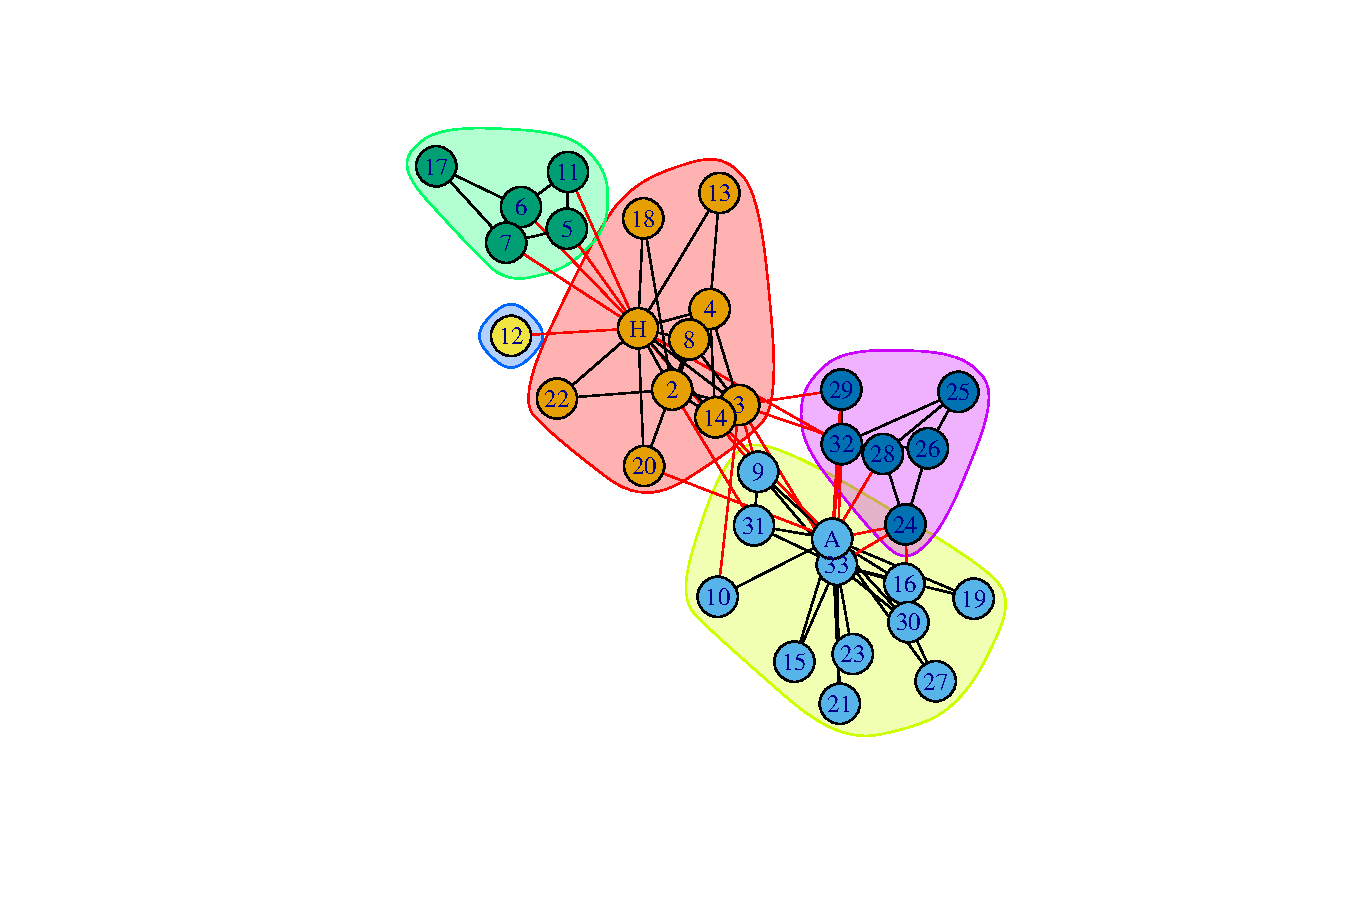
\includegraphics[width=.8\textwidth]{figures/unnamed-chunk-5-1} 

\end{knitrout}

\end{frame}

\begin{frame}[fragile]
  \frametitle{Stochastic block models -- examples of topology}
  \framesubtitle{Star network}

\begin{knitrout}\scriptsize
\definecolor{shadecolor}{rgb}{0.969, 0.969, 0.969}\color{fgcolor}\begin{kframe}
\begin{alltt}
\hlstd{pi} \hlkwb{<-} \hlkwd{matrix}\hlstd{(}\hlkwd{c}\hlstd{(}\hlnum{0.05}\hlstd{,}\hlnum{0.3}\hlstd{,}\hlnum{0.3}\hlstd{,}\hlnum{0}\hlstd{),}\hlnum{2}\hlstd{,}\hlnum{2}\hlstd{)}
\hlstd{star} \hlkwb{<-} \hlstd{igraph}\hlopt{::}\hlkwd{sample_sbm}\hlstd{(}\hlnum{100}\hlstd{, pi,} \hlkwd{c}\hlstd{(}\hlnum{4}\hlstd{,} \hlnum{96}\hlstd{))}
\hlkwd{plot}\hlstd{(star,} \hlkwc{vertex.label}\hlstd{=}\hlnum{NA}\hlstd{,} \hlkwc{vertex.color} \hlstd{=} \hlkwd{rep}\hlstd{(}\hlnum{1}\hlopt{:}\hlnum{2}\hlstd{,}\hlkwd{c}\hlstd{(}\hlnum{4}\hlstd{,}\hlnum{96}\hlstd{)))}
\end{alltt}
\end{kframe}
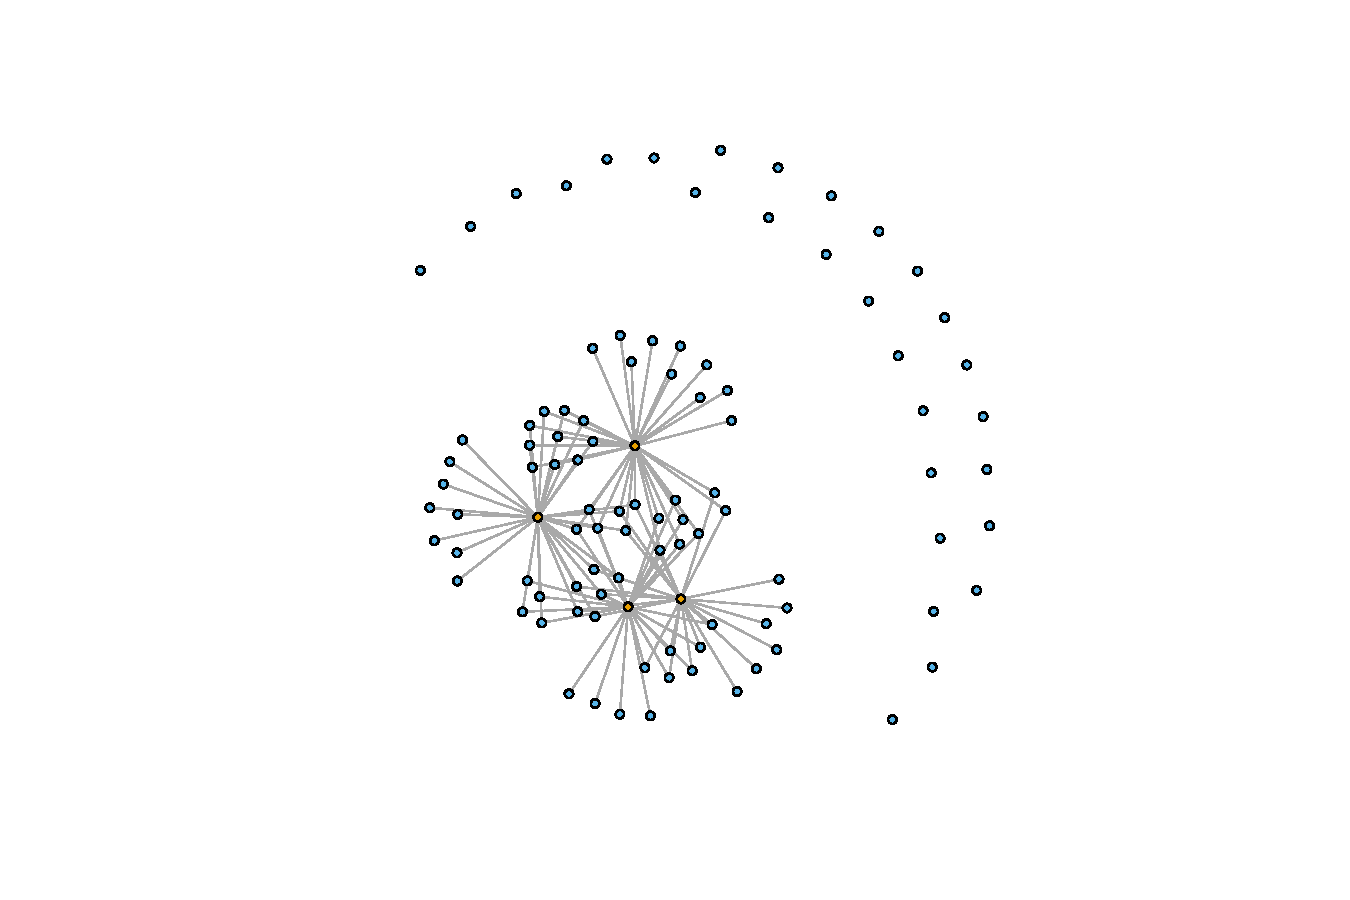
\includegraphics[width=.8\textwidth]{figures/unnamed-chunk-6-1} 

\end{knitrout}

\end{frame}

\begin{frame}
  \frametitle{Degree distributions}

  \begin{block}{Conditional degree distribution}
    The conditional degree distribution of a node $i\in q$ is
    \begin{equation*}
      D_i | i \in q \sim \mathrm{b}(n-1,\bar\pi) \approx \mathcal{P}(\lambda_q), \qquad \bar\pi_q = \sum_{\ell=1}^Q \alpha_\ell, \pi_{q\ell} \quad \lambda_q = (n-1)\bar\pi_q
    \end{equation*}
  \end{block}

  \vfill

  \begin{block}{Conditional degree distribution}
    The degree distribution of a node $i$ can be approximated by a mixture of Poisson distributions:
    \begin{equation*}
      \prob(D_i = k) = \sum_{q=1}^Q\alpha_q \exp{\set{-\lambda_q}} \ \frac{\lambda_q^k}{k !}
    \end{equation*}
  \end{block}

\end{frame}

\begin{frame}
  \frametitle{Likelihoods}

  \begin{block}{Complete-data loglikelihood}
    \vspace{-.5cm}
    \begin{equation*}
      \log L(\bX,\bZ) = \sum_{i,q} Z_{iq} \log \alpha_q + \sum_{i<j,q,\ell} Z_{iq}Z_{j\ell} \log \pi_{q\ell}^{X_{ij}} (1-\pi_{q\ell})^{1-X_{ij}}.
    \end{equation*}
  \end{block}

  \begin{block}{Conditional expectation of the complete-data loglikelihood}
    \vspace{-.5cm}
    \begin{equation*}
      \E_{\bZ|\bX} \big[\log L(\btheta;\bX,\bZ) \big] = \sum_{i,q} \tau_{iq} \log \alpha_q + \sum_{i<j,q,\ell} \eta_{ijq\ell} \log \pi_{q\ell}^{X_{ij}} (1-\pi_{q\ell})^{1-X_{ij}}
    \end{equation*}
      where $\tau_ {iq}, \eta_{ijq\ell}$ are the posterior probabilities:
      \begin{itemize}
        \item $\tau_{iq} = \prob(Z_{iq} = 1 | \bX) = \E \left[Z_{iq} | \bX\right].$
        \item $\eta_{ijq\ell} = \prob(Z_{iq}Z_{j\ell} = 1 | \bX) = \E \left[Z_{iq}Z_{j\ell} | \bX\right].$
      \end{itemize}
  \end{block}

\end{frame}

%% ==========================================================================
\subsection{Inference in SBM with variational EM}
%% ==========================================================================

\begin{frame}
  \frametitle{The EM strategy does not apply directly for SBM}

  \begin{block}{Ouch: another intractability problem}
    \begin{itemize}
      \item the $Z_{iq}$ are \alert{not independent} in the SBM framework\dots
      \item we cannot compute $\eta_{ijq\ell} = \prob(Z_{iq}Z_{j\ell} = 1 | \bX) = \E \left[Z_{iq}Z_{j\ell} | \bX\right]$,
      \item the conditional expectation $Q(\btheta)$, i.e. the main EM ingredient, is \alert{intractable}.
    \end{itemize}
  \end{block}

  \vfill

  \begin{block}{Solution: mean field approximation}
    Approximate $\eta_{ijq\ell}$ by $\tau_{iq}\tau_{j\ell}$, i.e., \alert{assume independence between $Z_{iq}$}\\

    $\rightsquigarrow$ This can be formalized in the variational framework
  \end{block}


\end{frame}

\begin{frame}
  \frametitle{Revisting the EM algorithm I}

  \begin{proposition}
    Consider a distribution $\mathbb{Q}$ for the $\set{Z_{iq}}$. We have
    \begin{equation*}
      \log L(\btheta; \bX) = \E_{\mathbb{Q}} [\log L(\btheta, \bX,\bZ)] + \mathcal{H}(\mathbb{Q}) + \mathrm{KL}(\mathbb{Q} \ | \ \prob(\bZ|\bX;\btheta)),
    \end{equation*}
    where $\mathcal{H}$ is the entropy and $\mathrm{KL}( \cdot| \cdot)$ is the Kullback-Leibler divergence:
    \begin{gather*}
      \mathcal{H}(\mathbb{Q}) = - \sum_z \mathbb{Q}(z) \log \mathbb{Q}(z) = - \E_\mathbb{Q} [\log \mathbb{Q} (Z)]\\
      \mathcal{KL}(\mathbb{Q} \ | \ \prob(\bZ|\bX;\btheta)) = \sum_z \mathbb{Q}(z) \log \frac{\mathbb{Q}(z)}{\prob(\bZ|\bX;\btheta)} = \E_\mathbb{Q} \left[\log \frac{\mathbb{Q}(z)}{\prob(\bZ|\bX;\btheta)}\right]\\
    \end{gather*}
  \end{proposition}
\end{frame}

\begin{frame}
  \frametitle{Revisting the EM algorithm II}
  Let
   \begin{equation*}
    J(\mathbb{Q},\btheta) \triangleq \E_{\mathbb{Q}}\left(\log L(\btheta ;\bX,\bZ)\right) + \mathcal{H}(\mathbb{Q})
\end{equation*}

  \vfill

  The steps in the EM algorithm may be viewed as:
  \begin{description}
    \item[Expectation step]: choose $\mathbb{Q}$ to maximize $J(\mathbb{Q};\btheta^{(t)})$\\[2ex]
      \alert{The solution is $\prob(\bZ|\bX;\btheta^{(t)})$}\\
    \item[Maximization step]: choose $\btheta$ to maximize $J(\mathbb{Q}^{(t)};\btheta$)\\[2ex]
      \alert{The solution maximizes $\E_{\bZ|\bX;\btheta^{(t)}}\left(\log L(\btheta ;\bX,\bZ)\right)$}
  \end{description}

\end{frame}

\begin{frame}
  \frametitle{Variational approximation for SBM}

    \begin{block}{Problem for SBM}
      $\prob(\bZ|\bX;\btheta^{(t)})$ cannot be computed thus the E-step cannot be solved.
  \end{block}

  \begin{block}{Idea}
      Choose $\mathbb{Q}$ in a class of function so that the E-step can be solved.
  \end{block}

  \begin{block}{Family of distribution that factorizes}
      We chose $\mathbb{Q}$ so as the $Z_{iq}$ are marginally independents:
      \begin{equation*}
        \mathbb{Q}(\bZ) = \prod_{i=1}^n \mathbb{Q}_i(Z_i) = \prod_{i=1}^n\prod_{q=1}^Q \tau_{iq}^{Z_{iq}},
      \end{equation*}
      where $\tau_{iq} =\mathbb{Q}_i(Z_{i} = q) = \E{Q}(Z_{iq})$, with $\sum_{q} \tau_{iq} = 1$ for all $i=1,\dots,n$.
  \end{block}

\end{frame}

\begin{frame}
  \frametitle{Variational EM for SBM: the criterion}

  \begin{block}{Lower bound of the loglikehood}
  Since $\mathbb{Q}$ is an approximation of $\prob(\bZ|\bX)$, the Kullback-Leibler divergence is non-negative and
    \begin{equation*}
      \log L(\btheta; \bX) \geq \E_{\mathbb{Q}} [\log L(\btheta, \bX,\bZ)] + \mathcal{H}(\mathbb{Q}) = J(\mathbb{Q},\btheta).
    \end{equation*}
  \end{block}

  For the SBM,
  \begin{equation*}
  J(\mathbb{Q},\btheta) = \sum_{i,q} \tau_{iq} \log \alpha_q + \sum_{i<j,q,\ell}  \tau_{iq}  \tau_{j\ell} \log b(X_{ij} ; \pi_{q\ell}) - \sum_{i,q} \tau_{iq} \log(\tau_{iq}),
  \end{equation*}

  $\rightsquigarrow$ we optimize the loglikelihood lower bound $J(\mathbb{Q},\btheta) = J(\boldsymbol\tau,\btheta)$ in $(\boldsymbol\tau, \btheta)$.

\end{frame}

\begin{frame}
  \frametitle{E and M steps for SBM}

  \begin{block}{Variational E-step}
    Maximizing $J(\boldsymbol\tau)$ for fixed $\btheta$, we find a fixed-point relationship:
    \begin{equation}
      \hat{\tau}_{iq} \varpropto \alpha_q \prod_{j} \prod_{\ell} b(X_{ij}, \pi_{q\ell})^{\hat{\tau}_{j\ell}}
    \end{equation}
  \end{block}

  \vfill

  \begin{block}{M-step}
    Maximizing $J(\btheta)$ for fixed $\boldsymbol\tau$, we find,
    \begin{equation}
\hat{\alpha}_q = \frac{1}{n}\sum_i \hat{\tau}_{iq} , \quad \hat\pi_{q\ell} = \frac{\sum_{i\neq j} \hat{\tau}_{iq}\hat{\tau}_{j\ell} X_{ij}}{\sum_{i\neq j} \hat{\tau}_{iq}\hat{\tau}_{j\ell}}.
\end{equation}
  \end{block}

\end{frame}

\begin{frame}
  \frametitle{Model selection}

  We use our lower bound of the  loglikelihood to compute an approximation of the ICL
  \begin{multline*}
  \mathrm{vICL}(Q) = \E_{\hat{\mathbb{Q}}} [\log L(\hat{\btheta)};\bX,\bZ] \\ - \frac{1}{2} \left(\frac{Q(Q+1)}{2} \log \frac{n(n-1)}{2} + (Q-1) \log (n) \right),
\end{multline*}
where
    \begin{equation*}
      \E_{\hat{\mathbb{Q}}} [\log L(\hat\btheta; \bX,\bZ)] = J(\hat{\boldsymbol\tau},\hat\btheta) - \mathcal{H}(\hat{\mathbb{Q}}).
    \end{equation*}

    The variational BIC is just
    \begin{equation*}
  \mathrm{vBIC}(Q) = J(\hat{\boldsymbol\tau},\hat\btheta) - \frac{1}{2} \left(\frac{Q(Q+1)}{2} \log \frac{n(n-1)}{2} + (Q-1) \log (n) \right).
    \end{equation*}

\end{frame}

\begin{frame}[fragile]
  \frametitle{Example on the French blogsphere (I)}

\begin{knitrout}\scriptsize
\definecolor{shadecolor}{rgb}{0.969, 0.969, 0.969}\color{fgcolor}\begin{kframe}
\begin{alltt}
\hlkwd{library}\hlstd{(blockmodels)}
\hlkwd{library}\hlstd{(sand)}

\hlstd{adj_blog} \hlkwb{<-} \hlkwd{upgrade_graph}\hlstd{(fblog)} \hlopt
    \hlkwd{as_adjacency_matrix}\hlstd{()} \hlopt
    \hlkwd{as.matrix}\hlstd{()}

\hlstd{mySBM_collection} \hlkwb{<-} \hlkwd{BM_bernoulli}\hlstd{(}
  \hlstr{"SBM_sym"}\hlstd{,}
  \hlstd{adj_blog,} \hlkwc{verbosity} \hlstd{=} \hlnum{0}\hlstd{,}
  \hlkwc{plotting} \hlstd{=} \hlstr{"figures/ICL_fblog.pdf"}
\hlstd{)}
\hlstd{mySBM_collection}\hlopt{$}\hlkwd{estimate}\hlstd{()}
\end{alltt}
\end{kframe}






































































\end{knitrout}

\end{frame}

\begin{frame}[fragile]
  \frametitle{Example on the French blogsphere (II)}

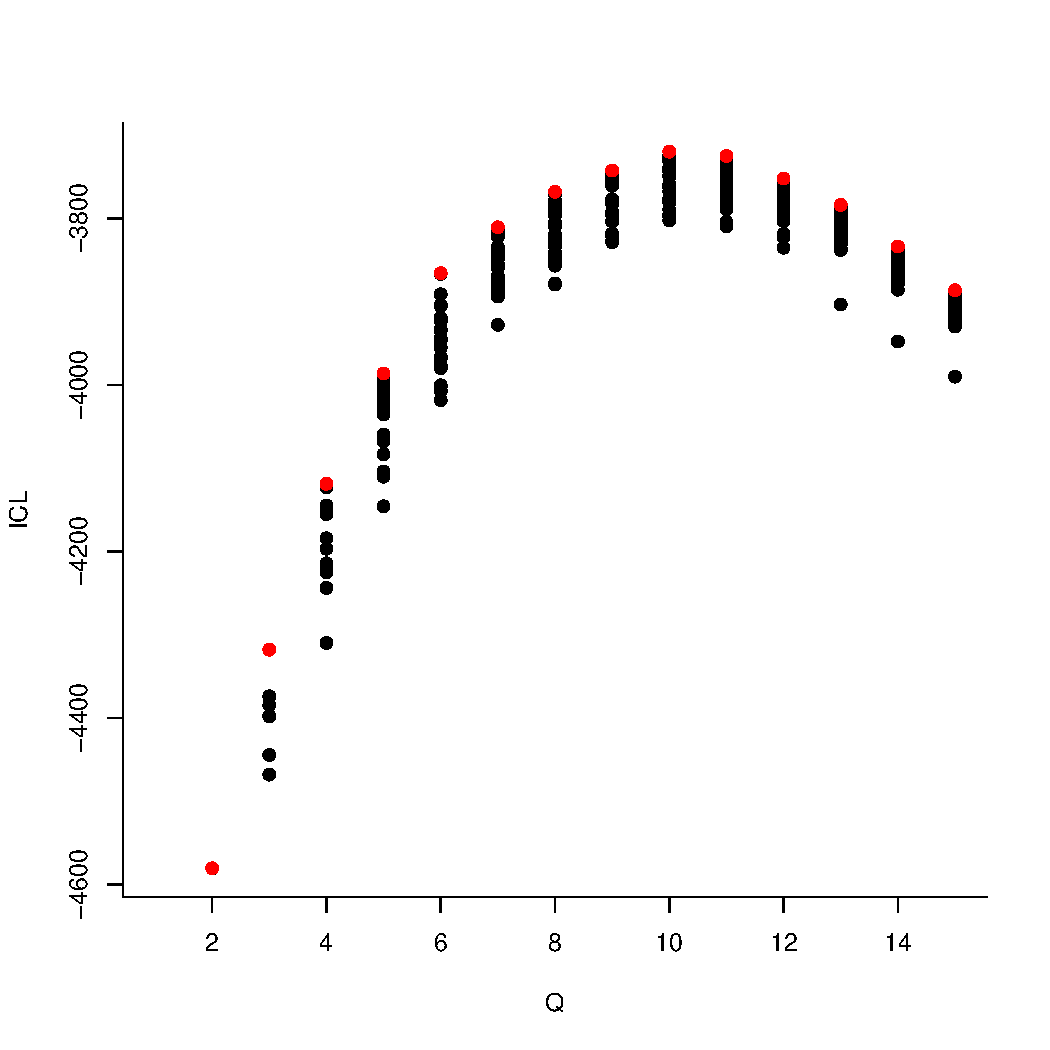
\includegraphics[width=.7\textwidth]{figures/ICL_fblog}

\end{frame}

\begin{frame}[fragile]
  \frametitle{Example on the French blogsphere (III)}

\begin{knitrout}\scriptsize
\definecolor{shadecolor}{rgb}{0.969, 0.969, 0.969}\color{fgcolor}\begin{kframe}
\begin{alltt}
\hlkwd{library}\hlstd{(Matrix)}
\hlstd{clusters} \hlkwb{<-}
  \hlkwd{apply}\hlstd{(mySBM_collection}\hlopt{$}\hlstd{memberships[[}\hlnum{10}\hlstd{]]}\hlopt{$}\hlstd{Z,} \hlnum{1}\hlstd{, which.max)}
\hlkwd{image}\hlstd{(}\hlkwd{Matrix}\hlstd{(adj_blog[}\hlkwd{order}\hlstd{(clusters),} \hlkwd{order}\hlstd{(clusters)]))}
\end{alltt}
\end{kframe}
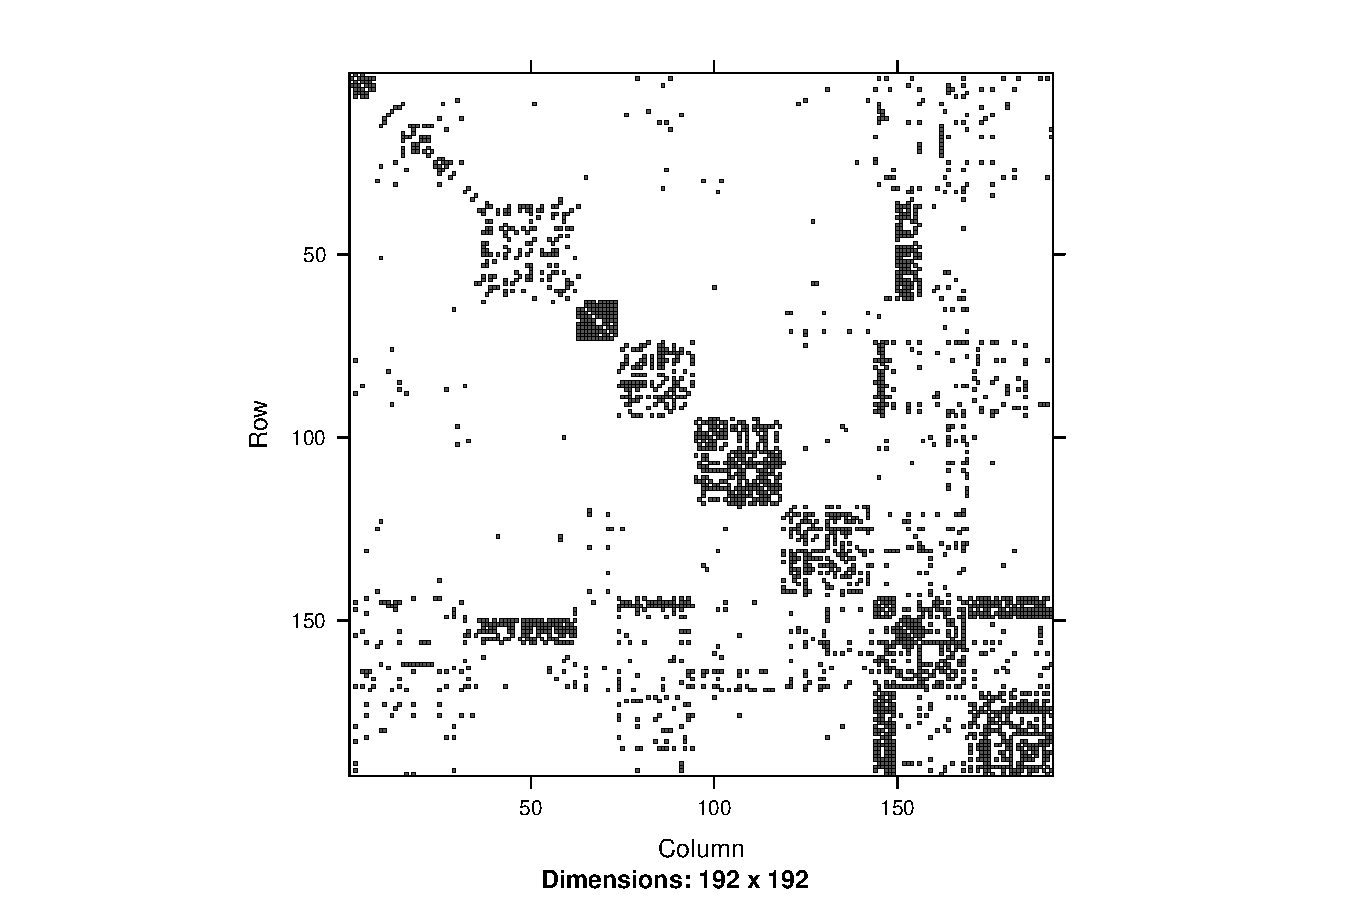
\includegraphics[width=.8\textwidth]{figures/example_blockmodels_3-1} 

\end{knitrout}

\end{frame}


\begin{frame}[fragile,allowframebreaks]
  \frametitle{Example on the French blogsphere (IV)}

\begin{knitrout}\scriptsize
\definecolor{shadecolor}{rgb}{0.969, 0.969, 0.969}\color{fgcolor}\begin{kframe}
\begin{alltt}
\hlkwd{library}\hlstd{(RColorBrewer); pal} \hlkwb{<-} \hlkwd{brewer.pal}\hlstd{(}\hlnum{10}\hlstd{,} \hlstr{"Set3"}\hlstd{)}

\hlstd{g} \hlkwb{<-} \hlkwd{graph_from_adjacency_matrix}\hlstd{(}
  \hlstd{adj_blog,}
  \hlkwc{mode} \hlstd{=} \hlstr{"undirected"}\hlstd{,}
  \hlkwc{weighted} \hlstd{=} \hlnum{TRUE}\hlstd{,}
  \hlkwc{diag} \hlstd{=} \hlnum{FALSE}
\hlstd{)}
\hlkwd{V}\hlstd{(g)}\hlopt{$}\hlstd{class} \hlkwb{<-} \hlstd{clusters}
\hlkwd{V}\hlstd{(g)}\hlopt{$}\hlstd{size} \hlkwb{<-} \hlnum{5}
\hlkwd{V}\hlstd{(g)}\hlopt{$}\hlstd{frame.color} \hlkwb{<-} \hlstr{"white"}
\hlkwd{V}\hlstd{(g)}\hlopt{$}\hlstd{color} \hlkwb{<-} \hlstd{pal[}\hlkwd{V}\hlstd{(g)}\hlopt{$}\hlstd{class]}
\hlkwd{V}\hlstd{(g)}\hlopt{$}\hlstd{label} \hlkwb{<-} \hlstr{""}
\hlkwd{E}\hlstd{(g)}\hlopt{$}\hlstd{arrow.mode} \hlkwb{<-} \hlnum{0}

\hlkwd{par}\hlstd{(}\hlkwc{mar} \hlstd{=}\hlkwd{c}\hlstd{(}\hlnum{0}\hlstd{,}\hlnum{0}\hlstd{,}\hlnum{0}\hlstd{,}\hlnum{0}\hlstd{))}
\hlkwd{plot}\hlstd{(g,} \hlkwc{edge.width}\hlstd{=}\hlkwd{E}\hlstd{(g)}\hlopt{$}\hlstd{weight)}
\end{alltt}
\end{kframe}

{\centering 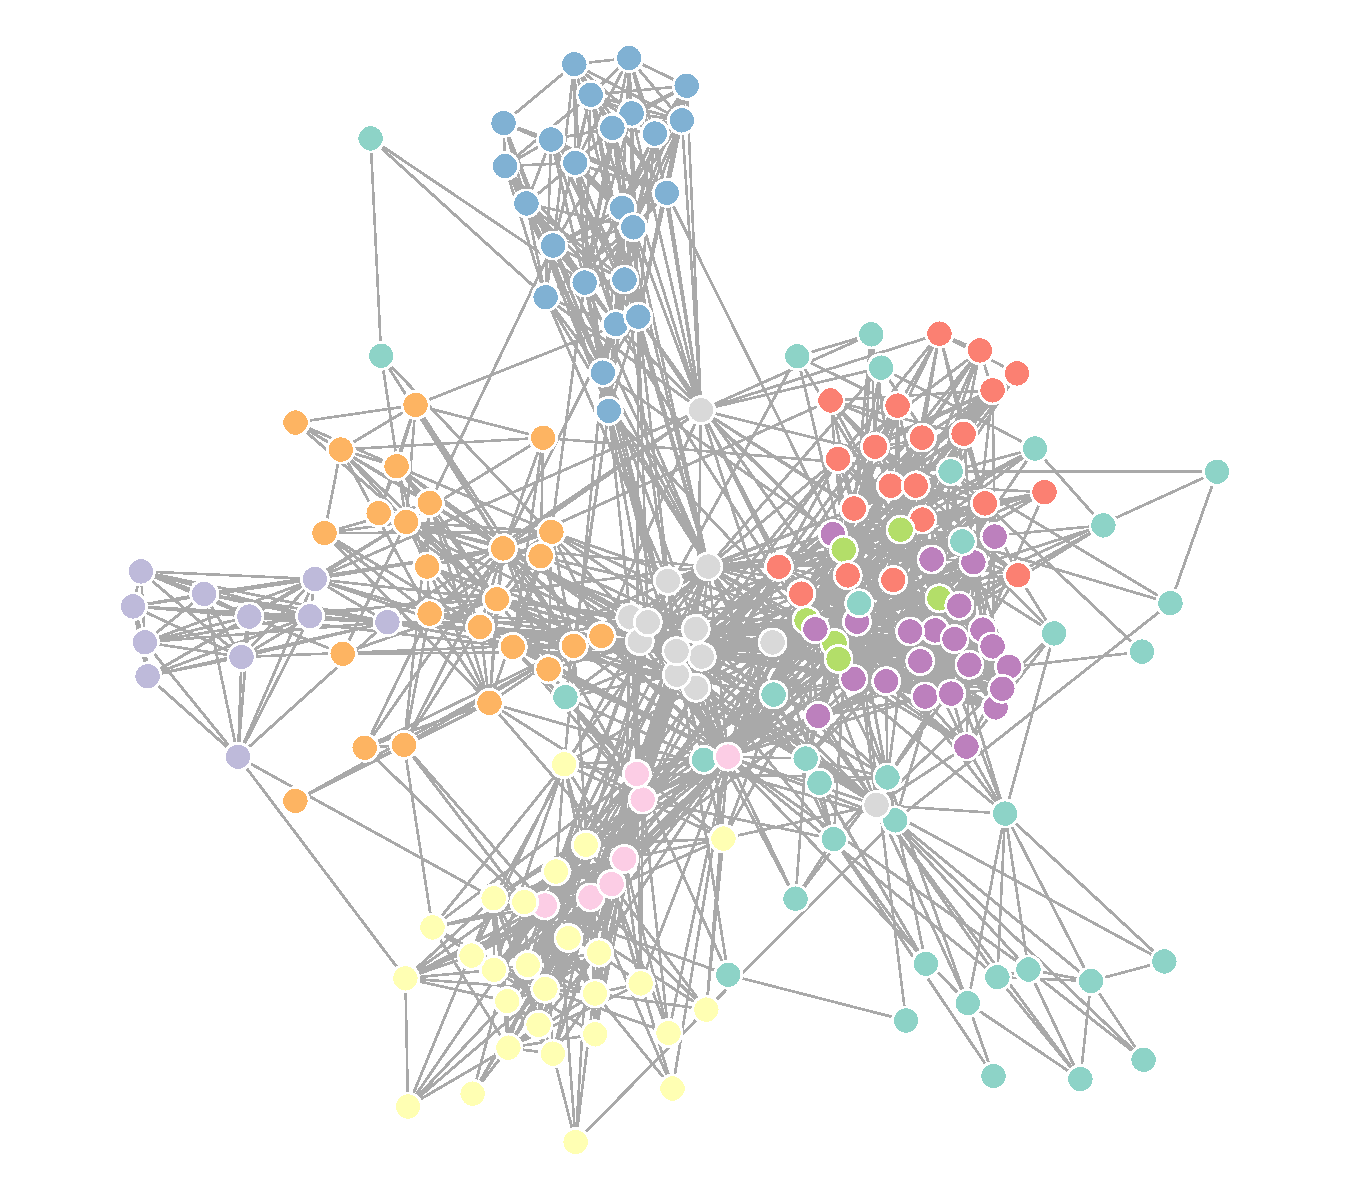
\includegraphics[width=.8\textwidth]{figures/example_blockmodels_4-1} 

}



\end{knitrout}

\end{frame}

\end{document}
